\documentclass[10pt,journal,compsoc]{IEEEtran}
\usepackage{graphicx}
\usepackage{balance}  
\usepackage[utf8x]{inputenc}
\usepackage[colorinlistoftodos]{todonotes}
\usepackage{adjustbox}
%\usepackage{hyperref}
\usepackage{microtype}
\usepackage{pgfplots} 
\usepackage{multirow}
\usepackage{multicol}
\usepackage{algorithm}
\usepackage{url}
\usepackage{wrapfig}
\usepackage{lipsum}
\usepackage{tikz}
\usepackage{pgfplots}
\usepackage{textcomp}
\usetikzlibrary{shapes,arrows,fit,chains}
\usepackage{algorithm}
\usepackage{algpseudocode}
\usepackage{pgfplots, pgfplotstable}
\usepackage{tikz}
\usepackage{listings}
\usepackage{xcolor}
\usetikzlibrary{patterns}
\usetikzlibrary{backgrounds}
\usepackage{booktabs}
\usepackage{verbatim}
\usepackage{fancyvrb}
\usepackage{verbatimbox,lipsum}
\usepackage{listings}
\usepgfplotslibrary{groupplots}

%\pgfplotsset{compat=1.9}
%\pgfplotsset{compat=1.12}



\newcommand{\definevariableobject}[1] {\textcolor{black}{ 
		\ttfamily\bfseries\textcolor{red}{\ #1}}
} 
\newcommand{\definevariable}[1] {\textcolor{black}{ 
		\ttfamily\bfseries\ #1}
} 
\definecolor{copper}{cmyk}{0,0.9,0.9,0.2}
\colorlet{lightgray}{black!25}
\colorlet{darkgray}{black!75}

\usepackage{xcolor}
\definecolor{tug}{RGB}{247,1,70}
\definecolor{tugb}{RGB}{120,137,251}


\definecolor{color1}{RGB}{100,149,237} % corn flower blue
\definecolor{color2}{RGB}{153,153,153} % light gray
\definecolor{color3}{RGB}{0,0,0} % black
\definecolor{color4}{RGB}{255,165,0} % orange
\definecolor{color5}{RGB}{255,69,0} % orange red
\definecolor{color6}{RGB}{77,77,77} % dark gray
\definecolor{color7}{RGB}{31,119,180}
\definecolor{color8}{RGB}{7,77,125}

% Enable this two commands when you want to extract diagrams in extra files, then run "make"
\usetikzlibrary{external}
\tikzexternalize[prefix=plots/] %  activate

\newcommand{\showvaluewrite}[8]{
  \ifthenelse{
    \equal{#1}{#2} \OR
    \equal{#1}{#3} \OR
    \equal{#1}{#4} \OR
    \equal{#1}{#5} \OR
    \equal{#1}{#6} \OR
    \equal{#1}{#7} \OR
    \equal{#1}{#8} 
  }{\pgfkeys{/tikz/coordinate}}{}
}

\newcommand{\showvalue}[9]{
  \ifthenelse{
    \equal{#1}{#2} \OR
    \equal{#1}{#3} \OR
    \equal{#1}{#4} \OR
    \equal{#1}{#5} \OR
    \equal{#1}{#6} \OR
    \equal{#1}{#7} \OR
    \equal{#1}{#8} \OR
    \equal{#1}{#9} 
  }{\pgfkeys{/tikz/coordinate}}{}
}


% *** CITATION PACKAGES ***
%
\ifCLASSOPTIONcompsoc
  % IEEE Computer Society needs nocompress option
  % requires cite.sty v4.0 or later (November 2003)
  \usepackage[nocompress]{cite}
\else
  % normal IEEE
  \usepackage{cite}
\fi

% *** GRAPHICS RELATED PACKAGES ***
%
\ifCLASSINFOpdf
  % \usepackage[pdftex]{graphicx}
  % declare the path(s) where your graphic files are
  % \graphicspath{{../pdf/}{../jpeg/}}
  % and their extensions so you won't have to specify these with
  % every instance of \includegraphics
  % \DeclareGraphicsExtensions{.pdf,.jpeg,.png}
\else
  % or other class option (dvipsone, dvipdf, if not using dvips). graphicx
  % will default to the driver specified in the system graphics.cfg if no
  % driver is specified.
  % \usepackage[dvips]{graphicx}
  % declare the path(s) where your graphic files are
  % \graphicspath{{../eps/}}
  % and their extensions so you won't have to specify these with
  % every instance of \includegraphics
  % \DeclareGraphicsExtensions{.eps}
\fi

\makeatletter
\def\endthebibliography{%
	\def\@noitemerr{\@latex@warning{Empty `thebibliography' environment}}%
	\endlist
}
\makeatother

%\theoremstyle{definition}
%\newtheorem{findings}{Findings}


\hyphenation{op-tical net-works semi-conduc-tor}

\begin{document}

\title{Understanding and Benchmarking the Impact of Complex Object Implementations for Big Data Systems}

\author{Saeed Fathollahzadeh, Kia Teymourian, Chris Jermaine 
	\IEEEcompsocitemizethanks{
		\IEEEcompsocthanksitem 
		Saeed Fathollahzadeh is with the Department of Computer Science, Graz University of Technology, Graz, Austria.\protect\\ E-mail: s.fathollahzadeh@student.tugraz.at
		\IEEEcompsocthanksitem Kia Teymourian is with the Department of Computer Science, The University of Texas at Austin, TX, USA. \protect\\ E-mail: kiat@bu.edu
		\IEEEcompsocthanksitem Chris Jermaine is the Chair of Department of Computer Science, Rice University, Houston, TX, USA. \protect\\ E-mail: cmj4@rice.edu}	
\thanks{Manuscript received April 19, 2005; revised August 26, 2015.}}


% The paper headers
\markboth{Fathollahzadeh, et al: Understanding and Benchmarking the Impact of Complex Object Implementations for Big Data Systems}%
{Shell \MakeLowercase{\textit{et al.}}: Bare Demo of IEEEtran.cls for Computer Society Journals}

\IEEEtitleabstractindextext{%
\begin{abstract}

\end{abstract}

\begin{IEEEkeywords}
Computer Society, IEEE, IEEEtran, journal, \LaTeX, paper, template.
\end{IEEEkeywords}}
% \tikzsetnextfilename{Exp0_serialize_benchmark}
%     \begin{figure*}[h]
%         \centering
%         \begin{tikzpicture}[scale=1, node distance=6.0mm]
    \newcommand{\myaddplot}[4]{
        \addplot[color=#4,mark=#3,discard if single={#1}]
        table[ y=#2, col sep=comma, x=object_level] {results/Exp0_benchmark.dat};
        \label{#1}
    };

    \newcommand{\addDiagramExpThree}[2]{
        \myaddplot{ProtoBuf}{deserialization_time}{*}{color1};        
        \myaddplot{FlatBuf}{deserialization_time}{square*}{color2};
        \myaddplot{Boost}{deserialization_time}{square*}{color3};
        \myaddplot{Hand-coded}{deserialization_time}{triangle}{color6};
        \myaddplot{inPlace}{deserialization_time}{triangle*}{color5};

        \node [draw=none,inner sep=1, font=\Large] at (rel axis cs: 0.3,0.65){\shortstack[l]{
            \ref{ProtoBuf} ProtoBuf \\
            \ref{FlatBuf} FlatBuf \\
            \ref{Boost} Boost \\
            \ref{Hand-coded} Hand-coded \\
            \ref{inPlace} inPlace
        }};
   };

   
   \pgfplotsset{
	discard if single/.style n args={1}{
		x filter/.code={
			\edef\tempa{\thisrow{baseline}}
			\edef\tempb{#1}
			\ifx\tempa\tempb
			\else
			\def\pgfmathresult{inf}
			\fi
		}
	}
};

    \begin{axis}
        [
        ymode=log,    
        ymin=0,
        ymax=15,
        y tick label style={/pgf/number format/1000 sep={}},   
        scaled y ticks=false,
        scaled x ticks=false,
        tick label style={/pgf/number format/fixed},
        enlarge x limits=0.03,
        ylabel={Latency[$\mu s$]},
        xlabel={$\#$ Objects Level},
        xtick pos=left,
        ytick pos=left,
        ytick align=outside,
        xtick align=outside,
        yticklabel style = {font=\Large},
        ylabel style = {font=\Large},
        xticklabel style = {font=\Large},
        xtick=data,
        xtick={1,2,3,4,5},
        xticklabels={1,2,4,8,16},
        xlabel style = {font=\Large, yshift=-7pt},
        height=0.6\columnwidth,
        width=\columnwidth,
        grid=both,
        grid style=dotted,
        minor grid style={gray!50},
        every axis plot/.append style={line width=1pt,mark options={scale=1.7,solid}},
        ]
        \addDiagramExpThree{}{};

    \end{axis}

\end{tikzpicture}
%         \caption{Benchmark-De/Serialize}
% \end{figure*}

% \tikzsetnextfilename{Exp0_metadata}
%     \begin{figure*}[h]
%         \centering
%         \begin{tikzpicture}[scale=1, node distance=6.0mm]
    \newcommand{\myaddplot}[4]{
        \addplot[color=#4,mark=#3,discard if single={#1},dotted, line cap=round, mark options={scale=2,solid, #4,fill=#4}]
        table[ y=#2, col sep=comma, x=object_level] {results/Exp0_benchmark.dat};
        \label{#1}
    };

    \newcommand{\addDiagramExpThree}[2]{
        \myaddplot{FlatBuf}{meta_data}{triangle*}{black};
        \myaddplot{ProtoBuf}{meta_data}{*}{black};        
        \myaddplot{Boost}{meta_data}{diamond*}{black};
        \myaddplot{Hand-coded}{meta_data}{pentagon*}{black};
        \myaddplot{inPlace}{meta_data}{square*}{black};

        \node [draw=none,inner sep=1, font=\Large] at (rel axis cs: 0.3,0.8){\shortstack[l]{
            \ref{ProtoBuf} ProtoBuf \\ \\
            \ref{FlatBuf} FlatBuf \\ \\
            \ref{Boost} Boost \\ \\
            \ref{Hand-coded} Hand-coded \\ \\
            \ref{inPlace} inPlace
        }};
   };

   
   \pgfplotsset{
	discard if single/.style n args={1}{
		x filter/.code={
			\edef\tempa{\thisrow{baseline}}
			\edef\tempb{#1}
			\ifx\tempa\tempb
			\else
			\def\pgfmathresult{inf}
			\fi
		}
	}
};

    \begin{axis}
        [
        %ymode=log,    
        ymin=0,
        %ymax=15,
        y tick label style={/pgf/number format/1000 sep={}},   
        scaled y ticks=false,
        scaled x ticks=false,
        tick label style={/pgf/number format/fixed},
        enlarge x limits=0.03,
        ylabel={Meta Data Size[byte]},
        xlabel={$\#$ Objects Level},
        xtick pos=left,
        ytick pos=left,
        ytick align=outside,
        xtick align=outside,
        yticklabel style = {font=\Large},
        ylabel style = {font=\Large, yshift=5pt},
        xticklabel style = {font=\Large},
        xtick=data,
        xtick={1,2,3,4,5},
        xticklabels={1,2,4,8,16},
        xlabel style = {font=\Large, yshift=-7pt},
        height=\columnwidth,
        width=\columnwidth,
        grid=both,
        grid style=dotted,
        minor grid style={gray!50},
        every axis plot/.append style={line width=1pt,mark options={scale=10,solid}},        
        ]
        \addDiagramExpThree{}{};

    \end{axis}

\end{tikzpicture}
%         \caption{Benchmark-Deserialize}
% \end{figure*}

% \tikzsetnextfilename{Exp1_write_single}
%     \begin{figure*}[h]
%         \centering
%         \makeatletter
\newcommand\resetstackedplots{
	\makeatletter
	\pgfplots@stacked@isfirstplottrue
	\makeatother
	\addplot [forget plot,draw=none] coordinates{({HandcodedCPP},0.1) ({inPlaceCPP},0.1) ({ProtoBufCPP},0.1) ({FlatBufCPP},0.1)  ({BoostBinaryCPP},0.1) ({BoostCPP},0.1)  ({BsonCPP},0.1) 
	({MessagePackRust},0.1) ({BincodeRust},0.1)  ({JsonRust},0.1) ({FlexBufRust},0.1) ({BsonRust},0.1) 
	({ByteBufferJava},0.1) ({KryoJava},0.1) ({ProtoBufJava},0.1) ({FlatBufJava},0.1) ({DefaultJava},0.1) ({BsonJava},0.1)  ({JsonJava},0.1) ({Json+GzipJava},0.1)};
}
\makeatother


\begin{tikzpicture}
	\newcommand{\myaddplot}[8]{
	   \addplot[white,xshift=#2,draw=#5,line width=0.15pt, fill=#3, discard if single={#1}{#4}{#8}, postaction={pattern=#6,pattern color=#5}] 
	   table[ y=time, col sep=comma, x=baseline] {results/Exp1_write_single.dat};
	   \label{#4#1}
   };  

   \newcommand{\myaddplotnan}[9]{
	   \addplot[xshift=#2,draw=#9,line width=0.15pt, fill=#3, discard if single={#1}{#4}{#8}, %postaction={pattern=#6,pattern color=#5},
	   visualization depends on={value \thisrow{baseline} \as \xbaseline},
	   every node near coord/.append style={		  
		   check for zeronan/.code={
			   \pgfkeys{/pgf/fpu=true}
			   \showvalue{\xbaseline}{HandcodedCPP}{inPlaceCPP}{FlatBufCPP}{}{MessagePackRust}{BincodeRust}{JsonRust}{}{}
			   \pgfkeys{/pgf/fpu=false}
		   },
		   check for zeronan,
	   }  
	   ] 
	   table[ y=time, col sep=comma, x=baseline] {results/Exp1_write_single.dat};	  
	   \label{#4#1}
   };  
   
   \newcommand{\myaddplots}[6]{	   
	\addplot[xshift=#2,draw=#5,line width=0.15pt, fill=#3, discard if single={#1}{#4}{#6},
		forget plot,
		nodes near coords custom=1,
		nodes near coords={\pgfmathprintnumber[precision=1]{\pgfplotspointmeta}},
		every node near coord/.append style={
			black,			
			xshift=-10pt,
			anchor=west
		}
	] 
	table[ y=time, col sep=comma, x=baseline] {results/Exp1_write_single.dat};	
   };   
   
   \newcommand{\addDiagramExpOne}[9]{	
	\nextgroupplot[
		width=#4,		
		ytick=#5,
		yticklabels =#5,
		y axis line style={opacity=#6},
		#7,
		axis y line*=#8,
		%xlabel=#9,				
		] 
		\resetstackedplots	
		\myaddplot{True}{-6}{black}{IO}{black}{none}{I/O Time(taskset True)}{#1};
  		\myaddplotnan{True}{-6}{white}{CPU}{black}{north east lines}{CPU Time(taskset True)}{#1}{black};
		\myaddplots{True}{-6}{white}{Total}{none}{#1};
	    \resetstackedplots	 
		\myaddplot{False}{6}{gray!135}{IO}{gray!135}{none}{I/O Time(taskset False)}{#1};  
	    \myaddplotnan{False}{6}{lightgray!85}{CPU}{lightgray!85}{north west lines}{CPU Time(taskset False)}{#1}{black};
		\myaddplots{False}{6}{white}{Total}{none}{#1};
   };     

  \pgfplotsset{
	   discard if single/.style n args={3}{
		   x filter/.code={
			   \edef\tempa{\thisrow{taskset}}
			   \edef\tempb{#1}
			   \ifx\tempa\tempb
					   \edef\tempe{\thisrow{execution}}
					   \edef\tempf{#2}
					   \ifx\tempe\tempf	
					   	%%%%%%%%%%%%%%%%%%%
						   \edef\tempg{\thisrow{language}}
						   \edef\temph{#3}
						   \ifx\tempg\temph	
						   		%%%%%%%%%%%%%%%%%
								    \edef\tempi{\thisrow{platform}}
								    \edef\tempj{Single}
								    \ifx\tempi\tempj												   
								    \else
								    \def\pgfmathresult{inf}
								    \fi      
								%%%%%%%%%%%%%%%%%
						   \else
						   \def\pgfmathresult{inf}
						   \fi      
						%%%%%%%%%%%%%%%%%%%	
					   \else
					   \def\pgfmathresult{inf}
					   \fi      
			   \else
			   \def\pgfmathresult{inf}
			   \fi			
		   }
	   },
	   nodes near coords custom/.style={
		large value/.style={                    
			rotate=90,
			anchor=east,			
		},
		small value/.style={
			rotate=90,
			anchor=east,
		},
		every node near coord/.style={
		  font=\scriptsize,
		  inner sep=0.5mm,
		  /pgf/number format/1000 sep={},
		  check for zero/.code={%
			\pgfkeys{/pgf/fpu=true}
			\pgfmathparse{\pgfplotspointmeta-1}
			\pgfmathfloatifflags{\pgfmathresult}{0}{
				\pgfkeys{/tikz/coordinate}
			}{
				\begingroup                      
					\pgfkeys{/pgf/fpu}%
					\pgfmathparse{\pgfplotspointmeta<#1}%
					\global\let\result=\pgfmathresult
				\endgroup
				\pgfmathfloatcreate{1}{1.0}{0}%
				\let\ONE=\pgfmathresult
				\ifx\result\ONE
					% AH : our condition 'y < #1' is met.
					\pgfkeysalso{/pgfplots/small value}%
				\else
					% ok, proceed as usual.
					\pgfkeysalso{/pgfplots/large value}%
				\fi
			}
			\pgfkeys{/pgf/fpu=false}
		  },
		  check for zero,
		},
	},   
   };
   %%%%%%%%%%%%%%%%%%%%%%%%%%%%%%%%%%%%%%%%%%%%%%%%
   \begin{groupplot}[
		group style={
			group size=3 by 1,
			xlabels at=edge bottom,
			ylabels at=edge left,
			horizontal sep=0pt,
			vertical sep=0pt,
			/pgf/bar width=12pt
		},			
		axis line style={gray},
		ybar stacked,        
		ymode=log,
		ymin=0.2,
		ymax=100,
		scaled y ticks=false,		  
		enlarge y limits={0.15,upper},		
		ylabel={Execution Time [min]},		   
		ytick align=inside,
		xtick align=outside,			
		xtick pos=left,
		ytick pos=left,
		yticklabel style = {font=\footnotesize},
		ylabel style = { yshift=-12pt},
		xticklabel style = {font=\footnotesize},
		x label style={yshift=-20pt},
		xtick=data,
		height=0.7\columnwidth,  
		symbolic x coords={ HandcodedCPP, inPlaceCPP, ProtoBufCPP, FlatBufCPP, BoostBinaryCPP, BoostCPP, BsonCPP, MessagePackRust,BincodeRust, JsonRust, FlexBufRust, BsonRust,ByteBufferJava,KryoJava,ProtoBufJava,FlatBufJava,DefaultJava,BsonJava,JsonJava, Json+GzipJava},
		%
		xticklabels={HandCoded, , ProtoBuf, , BoostBinary, , BSON, ,Bincode, , FlexBuf, ,ByteBuffer,,ProtoBuf,,Default,,JSON, },  
		%
		extra x ticks={inPlaceCPP,FlatBufCPP,BoostCPP,MessagePackRust,JsonRust,BsonRust,KryoJava,FlatBufJava,BsonJava,Json+GzipJava},
		extra x tick labels={InPlace,FlatBuf,BoostText,MessagePack,JSON,BSON,Kryo,FlatBuf,BSON,JSON+Gzip},
		%
		every extra x tick/.style={major tick length=18pt, xtick align=outside},
		point meta=rawy,    		
		nodes near coords={\pgfmathprintnumber[fixed,assume math mode=true,precision=1]{\pgfplotspointmeta}},
		nodes near coords custom={1}, 
		legend image code/.code={\draw [#1] (-0.2cm,-0.1cm) rectangle (0.20cm,0.20cm); },
		xticklabel style={name=T\ticknum}			
]
\addDiagramExpOne{CPP}{tugb}{color7}{0.48\textwidth}{{10,100}}{1}{{enlarge x limits=0.12,}}{left}{C++};		
\node [draw=none,inner sep=0, font=\footnotesize, anchor=west](leg1) at (rel axis cs: 0.1,0.77) {\shortstack[l]{
		\ref{CPUTrue} CPU Time (taskset True) \\ 
		\ref{IOTrue} I/O Time (taskset True) \\
		\ref{CPUFalse} CPU Time (taskset False) \\ 
		\ref{IOFalse} I/O Time (taskset False) 				
}};
\addDiagramExpOne{Rust}{tugb}{color7}{0.40\textwidth}{\empty}{0}{{enlarge x limits=0.24,}}{left}{Rust};
\addDiagramExpOne{Java}{tugb}{color7}{0.55\textwidth}{\empty}{1}{{enlarge x limits=0.12,}}{right}{Java};
		
\end{groupplot}

\begin{scope}[decoration=brace]
	\pgfdecorationsegmentamplitude=5pt
	\draw[decorate] ($(T2.south east)+(25pt,0)$) -- ($(T0.south west)+(-25pt,0)$) node[midway,below=\pgfdecorationsegmentamplitude] {\footnotesize{C++}};
	\draw[decorate] ($(T4.south east)+(60pt,0)$) -- ($(T3.south west)+(5pt,0)$) node[midway,below=\pgfdecorationsegmentamplitude] {\footnotesize{Rust}};
	\draw[decorate] ($(T8.south east)+(58pt,0)$) -- ($(T5.south west)+(43pt,0)$) node[midway,below=\pgfdecorationsegmentamplitude] {\footnotesize{Java}};	
  \end{scope}
\end{tikzpicture}
%         \caption{Experiment1: Write times for 10M Tweet Objects (Single)}
% \end{figure*}

% \tikzsetnextfilename{Exp1_write_parallel}
%     \begin{figure*}[h]
%         \centering
%         \makeatletter
\newcommand\resetstackedplots{
	\makeatletter
	\pgfplots@stacked@isfirstplottrue
	\makeatother
	\addplot [forget plot,draw=none] coordinates{({HandcodedCPP},0.01) ({inPlaceCPP},0.01) ({FlatBufCPP},0.01) ({ProtoBufCPP},0.01) 
	({BoostCPP},0.01) ({BsonCPP},0.01) ({MessagePackRust},0.01) ({BincodeRust},0.01) ({JsonRust},0.01) ({FlexBufRust},0.01) ({BsonRust},0.01) ({Json+GzipJava},0.01) 
	({JsonJava},0.01) ({BsonJava},0.01) ({DefaultJava},0.01) ({ProtoBufJava},0.01) ({ByteBufferJava},0.01) ({FlatBufJava},0.01) ({KryoJava},0.01)};
}
\makeatother

\begin{tikzpicture}
	\newcommand{\myaddplot}[7]{
	   \addplot[xshift=#1,draw=#4,line width=0.15pt, fill=#2, discard if single={#3}{#7}, postaction={pattern=#5,pattern color=#4}] 
	   table[ y=time, col sep=comma, x=baseline] {results/Exp1_write.dat};
	   \label{#3#7}
   };  

   \newcommand{\myaddplotnan}[8]{
	   \addplot[xshift=#1,draw=#8,line width=0.15pt, fill=#2, discard if single={#3}{#7},
	   visualization depends on={value \thisrow{baseline} \as \xbaseline},
	   every node near coord/.append style={		  
		   check for zeronan/.code={
			   \pgfkeys{/pgf/fpu=true}
			   \showvalue{\xbaseline}{HandcodedCPP}{inPlaceCPP}{FlatBufCPP}{ProtoBufCPP}{BoostCPP}{MessagePackRust}{JsonRust}{FlexBufRust}{BsonRust};
			   \showvalue{\xbaseline}{BincodeRust}{BsonRust}{BsonJava}{DefaultJava}{}{}{}{}{}
			   \pgfkeys{/pgf/fpu=false}
		   },
		   check for zeronan,
	   }  
	   ] 
	   table[ y=time, col sep=comma, x=baseline] {results/Exp1_write.dat};	  
	   \label{#3#7}
   };  
   
   \newcommand{\myaddplots}[5]{	   
	\addplot[xshift=#1,draw=#4,line width=0.15pt, fill=#2, discard if single={#3}{#5},
		forget plot,
		nodes near coords custom=1,
		nodes near coords={\pgfmathprintnumber[precision=1]{\pgfplotspointmeta}},
		every node near coord/.append style={
			black,			
			xshift=-7pt,
			anchor=west
		}
	] 
	table[ y=time, col sep=comma, x=baseline] {results/Exp1_write.dat};	
   };   
   
   \newcommand{\addDiagramExpOne}[7]{	
	\nextgroupplot[
		width=#4,		
		yticklabels=#5,
		ytick=#6,
		#7
		]
		\resetstackedplots	
		\myaddplot{0}{#2}{IO}{#2}{none}{I/O Time(taskset True)}{#1};
  		\myaddplotnan{0}{#2!40}{CPU}{#2!40}{north east lines}{CPU Time(taskset True)}{#1}{#2};
		\myaddplots{0}{white}{Total}{none}{#1};
   };     

  \pgfplotsset{
	   discard if single/.style n args={2}{
		   x filter/.code={
		   \edef\tempe{\thisrow{execution}}
		   \edef\tempf{#1}
		   \ifx\tempe\tempf	
			   \edef\tempg{\thisrow{language}}
			   \edef\temph{#2}
			   \ifx\tempg\temph	
				    \edef\tempi{\thisrow{platform}}
				    \edef\tempj{Parallel}
				    \ifx\tempi\tempj												   
				    \else
				    \def\pgfmathresult{inf}
				    \fi      
			   \else
			   \def\pgfmathresult{inf}
			   \fi      
		   \else
		   \def\pgfmathresult{inf}
		   \fi      
	   }
	   },
	   nodes near coords custom/.style={
		large value/.style={                    
			rotate=90,
			anchor=east,			
		},
		small value/.style={
			rotate=90,
			anchor=east,
		},
		every node near coord/.style={
		  font=\scriptsize,
		  inner sep=0.5mm,
		  /pgf/number format/1000 sep={},
		  check for zero/.code={%
			\pgfkeys{/pgf/fpu=true}
			\pgfmathparse{\pgfplotspointmeta-0.1}
			\pgfmathfloatifflags{\pgfmathresult}{0}{
				\pgfkeys{/tikz/coordinate}
			}{
				\begingroup                      
					\pgfkeys{/pgf/fpu}%
					\pgfmathparse{\pgfplotspointmeta<#1}%
					\global\let\result=\pgfmathresult
				\endgroup
				\pgfmathfloatcreate{1}{0.1}{0}%
				\let\ONE=\pgfmathresult
				\ifx\result\ONE
					% AH : our condition 'y < #1' is met.
					\pgfkeysalso{/pgfplots/small value}%
				\else
					% ok, proceed as usual.
					\pgfkeysalso{/pgfplots/large value}%
				\fi
			}
			\pgfkeys{/pgf/fpu=false}
		  },
		  check for zero,
		},
	},   
   };
   %%%%%%%%%%%%%%%%%%%%%%%%%%%%%%%%%%%%%%%%%%%%%%%%
   \begin{groupplot}[
		group style={
			group size=3 by 1,
			xlabels at=edge bottom,
			ylabels at=edge left,
			horizontal sep=4pt,
			vertical sep=0pt,
			/pgf/bar width=8pt
		},			
		axis line style={gray},
		ybar stacked,        
		ymode=log,
		ymin=0.3,
		x tick label style={/pgf/number format/1000 sep=},
		ymax=400,		
		scaled y ticks=false,		  
		enlarge y limits={0.3,upper},		
		ylabel={Execution Time[s]},		   
		ytick align=inside,
		xtick align=outside,			
		xtick pos=left,
		ytick pos=left,
		yticklabel style = {font=\scriptsize},
		ylabel style = {font=\scriptsize, yshift=-12pt},
		xticklabel style = {font=\scriptsize, rotate=50, anchor=east, xshift=1pt, yshift=-1pt},
		x label style={yshift=-20pt},
		xtick=data,
		height=0.7\columnwidth,  
		symbolic x coords={ HandcodedCPP, inPlaceCPP, FlatBufCPP, ProtoBufCPP, BoostCPP, BsonCPP, MessagePackRust, BincodeRust, JsonRust, FlexBufRust, BsonRust, Json+GzipJava, JsonJava, BsonJava, DefaultJava, ProtoBufJava, ByteBufferJava, FlatBufJava, KryoJava},		   
		xticklabels={Handcoded, inPlace, FlatBuf, ProtoBuf, Boost, Bson, MessagePack, Bincode, Json, FlexBuf, Bson, Json+Gzip, Json, Bson, Default, ProtoBuf, ByteBuffer, FlatBuf, Kryo},  		   
		point meta=rawy,            
		nodes near coords={%
    		\pgfmathprintnumberto[fixed,assume math mode=true,precision=1]{\pgfplotspointmeta}{\myval}%
    		\pgfmathparse{\myval<=0.1?:\myval}\pgfmathresult%
		},
		nodes near coords custom={1}, 
		legend image code/.code={\draw [#1] (0cm,-0.1cm) rectangle (0.20cm,0.20cm); },
		xticklabel style={name=T\ticknum}			
]
\addDiagramExpOne{CPP}{tug}{color7}{0.21\textwidth}{{10,100,1000,10000}}{{10,100,1000}}{{enlarge x limits=0.15,}};	
\node [draw=none,inner sep=2, fill=lightgray, text width=0.12\textwidth,align=center,font=\scriptsize, anchor=west](leg1) at (rel axis cs: 0.00,0.965) {C++};
\node [draw=none,inner sep=0, font=\scriptsize, anchor=west](leg1) at (rel axis cs: 0.2,0.83) {\shortstack[l]{
		\ref{CPUCPP} CPU \\ \\ 
		\ref{IOCPP} IO 
}};

\addDiagramExpOne{Rust}{tugb}{color7}{0.19\textwidth}{}{}{{enlarge x limits=0.18,}};
\node [draw=none,inner sep=2, fill=lightgray, text width=0.1\textwidth,align=center,font=\scriptsize, anchor=west](leg1) at (rel axis cs: 0.00,0.965) {Rust};
\node [draw=none,inner sep=0, font=\scriptsize, anchor=west](leg1) at (rel axis cs: 0.2,0.83) {\shortstack[l]{
		\ref{CPURust} CPU \\ \\ 
		\ref{IORust} IO 
}};

\addDiagramExpOne{Java}{color4}{color7}{0.26\textwidth}{}{}{{enlarge x limits=0.14,}};
\node [draw=none,inner sep=2, fill=lightgray, text width=0.17\textwidth,align=center,font=\scriptsize, anchor=west](leg1) at (rel axis cs: 0.00,0.965) {Java};
\node [draw=none,inner sep=0, font=\scriptsize, anchor=west](leg1) at (rel axis cs: 0.7,0.83) {\shortstack[l]{
		\ref{CPUJava} CPU \\ \\ 
		\ref{IOJava} IO 
}};
\end{groupplot}
   
\end{tikzpicture}
%         \caption{Experiment1: Write times for 10M Tweet Objects (parallel)}
% \end{figure*}

% \tikzsetnextfilename{Exp2_seq_read_single}
%     \begin{figure*}[h]
%         \centering
%         \makeatletter
\newcommand\resetstackedplots{
	\makeatletter
	\pgfplots@stacked@isfirstplottrue
	\makeatother
	\addplot [forget plot,draw=none] coordinates{({HandcodedCPP},0.1) ({inPlaceCPP},0.1) ({ProtoBufCPP},0.1) ({FlatBufCPP},0.1)  ({BoostBinaryCPP},0.1) ({BoostCPP},0.1)  ({BsonCPP},0.1) 
	({MessagePackRust},0.1) ({BincodeRust},0.1)  ({JsonRust},0.1) ({FlexBufRust},0.1) ({BsonRust},0.1) 
	({ByteBufferJava},0.1) ({KryoJava},0.1) ({ProtoBufJava},0.1) ({FlatBufJava},0.1) ({DefaultJava},0.1) ({BsonJava},0.1)  ({JsonJava},0.1) ({Json+GzipJava},0.1)};
}
\makeatother


\begin{tikzpicture}
	\newcommand{\myaddplot}[8]{
	   \addplot[white,xshift=#2,draw=#5,line width=0.15pt, fill=#3, discard if single={#1}{#4}{#8}, postaction={pattern=#6,pattern color=#5}] 
	   table[ y=time, col sep=comma, x=baseline] {results/Exp2_read_single.dat};
	   \label{#4#1}
   };  

   \newcommand{\myaddplotnan}[9]{
	   \addplot[xshift=#2,draw=#9,line width=0.15pt, fill=#3, discard if single={#1}{#4}{#8}, visualization depends on={value \thisrow{baseline} \as \xbaseline},
	   every node near coord/.append style={		  
		   check for zeronan/.code={
			   \pgfkeys{/pgf/fpu=true}
			   \showvalue{\xbaseline}{inPlaceCPP}{FlatBufJava}{}{}{}{}{}{}{}
			   \pgfkeys{/pgf/fpu=false}
		   },
		   check for zeronan,
	   }  
	   ] 
	   table[ y=time, col sep=comma, x=baseline] {results/Exp2_read_single.dat};	  
	   \label{#4#1}
   };  
   
   \newcommand{\myaddplots}[6]{	   
	\addplot[xshift=#2,draw=#5,line width=0.15pt, fill=#3, discard if single={#1}{#4}{#6},
		forget plot,
		nodes near coords custom=1,
		nodes near coords={\pgfmathprintnumber[precision=2]{\pgfplotspointmeta}},
		every node near coord/.append style={
			black,			
			xshift=-7pt,
			anchor=west
		}
	] 
	table[ y=time, col sep=comma, x=baseline] {results/Exp2_read_single.dat};	
   };   
   
   \newcommand{\addDiagramExpOne}[9]{	
	\nextgroupplot[
		width=#4,		
		ytick=#5,
		yticklabels=#5,
		y axis line style={opacity=#6},
		#7,
		axis y line*=#8,
		%xlabel=#9,				
		]
		\resetstackedplots	
		\myaddplot{True}{-6}{colora}{IO}{black}{none}{I/O Time(taskset True)}{#1};
  		\myaddplotnan{True}{-6}{colorb}{CPU}{black}{north east lines}{CPU Time(taskset True)}{#1}{black};
		\myaddplots{True}{-6}{white}{Total}{none}{#1};
	    \resetstackedplots	 
		\myaddplot{False}{6}{colorc}{IO}{black}{none}{I/O Time(taskset False)}{#1};  
	    \myaddplotnan{False}{6}{colord}{CPU}{black}{north west lines}{CPU Time(taskset False)}{#1}{black};
		\myaddplots{False}{6}{white}{Total}{none}{#1};
   };     

  \pgfplotsset{
	   discard if single/.style n args={3}{
		   x filter/.code={
			   \edef\tempa{\thisrow{taskset}}
			   \edef\tempb{#1}
			   \ifx\tempa\tempb
					\edef\tempe{\thisrow{execution}}
					\edef\tempf{#2}
					\ifx\tempe\tempf	
					   	%
						\edef\tempg{\thisrow{language}}
						\edef\temph{#3}
						\ifx\tempg\temph	
							%
							\edef\tempi{\thisrow{platform}}
							\edef\tempj{Single}
								\ifx\tempi\tempj	
									%
									\edef\tempk{\thisrow{nrow}}
									\edef\templ{10000000}
									\ifx\tempk\templ
										%
										\edef\tempm{\thisrow{seq_rand}}
										\edef\tempn{Sequential}
										\ifx\tempm\tempn
										\else
										\def\pgfmathresult{inf}
							    		\fi 
										%	
									\else
									\def\pgfmathresult{inf}
							    	\fi  	
									%											   
							    \else
							    \def\pgfmathresult{inf}
							    \fi      
							%
						\else
						\def\pgfmathresult{inf}
						\fi      
						%
					\else
					\def\pgfmathresult{inf}
					\fi      
			   \else
			\def\pgfmathresult{inf}
			\fi			
		   }
	   },
	   nodes near coords custom/.style={
		large value/.style={                    
			rotate=90,
			anchor=east,			
		},
		small value/.style={
			rotate=90,
			anchor=east,
		},
		every node near coord/.style={
		  font=\scriptsize,
		  inner sep=0.5mm,
		  /pgf/number format/1000 sep={},
		  check for zero/.code={%
			\pgfkeys{/pgf/fpu=true}
			\pgfmathparse{\pgfplotspointmeta-0.11}
			\pgfmathfloatifflags{\pgfmathresult}{0}{
				\pgfkeys{/tikz/coordinate}
			}{
				\begingroup                      
					\pgfkeys{/pgf/fpu}%
					\pgfmathparse{\pgfplotspointmeta<#1}%
					\global\let\result=\pgfmathresult
				\endgroup
				\pgfmathfloatcreate{1}{0.1}{0}%
				\let\ONE=\pgfmathresult
				\ifx\result\ONE
					% AH : our condition 'y < #1' is met.
					\pgfkeysalso{/pgfplots/small value}%
				\else
					% ok, proceed as usual.
					\pgfkeysalso{/pgfplots/large value}%
				\fi
			}
			\pgfkeys{/pgf/fpu=false}
		  },
		  check for zero,
		},
	},   
   };
   %%%%%%%%%%%%%%%%%%%%%%%%%%%%%%%%%%%%%%%%%%%%%%%%
   \begin{groupplot}[
		group style={
			group size=3 by 1,
			xlabels at=edge bottom,
			ylabels at=edge left,
			horizontal sep=0pt,
			vertical sep=0pt,
			/pgf/bar width=12pt
		},			
		axis line style={gray},
		ybar stacked,        
		ymode=log,
		ymin=0.35,
		ymax=100,
		scaled y ticks=false,		  
		enlarge y limits={0.2,upper},		
		ylabel={Execution Time [min.]},		   
		ytick align=inside,
		xtick align=outside,			
		xtick pos=left,
		ytick pos=left,
		yticklabel style = {font=\footnotesize},
		ylabel style = {yshift=-12pt},
		xticklabel style = {font=\footnotesize},
		x label style={yshift=-20pt},
		xtick=data,
		height=0.4\columnwidth,
		width=\textwidth,  
		symbolic x coords={ HandcodedCPP, inPlaceCPP, ProtoBufCPP, FlatBufCPP, BoostBinaryCPP, BoostCPP, BsonCPP, MessagePackRust,BincodeRust, JsonRust, FlexBufRust, BsonRust,ByteBufferJava,KryoJava,ProtoBufJava,FlatBufJava,DefaultJava,BsonJava,JsonJava, Json+GzipJava},
		%
		xticklabels={HandCoded, , ProtoBuf, , BoostBinary, , BSON, ,Bincode, , FlexBuf, ,ByteBuffer, ,ProtoBuf, ,Default, ,JSON, },  
		%
		extra x ticks={inPlaceCPP,FlatBufCPP,BoostCPP,MessagePackRust,JsonRust,BsonRust,KryoJava,FlatBufJava,BsonJava,Json+GzipJava},
		extra x tick labels={InPlace,FlatBuf,BoostText,MessagePack,JSON,BSON,Kryo,FlatBuf,BSON,JSON+Gzip},
		%
		every extra x tick/.style={major tick length=18pt, xtick align=outside},
		point meta=rawy,            
		nodes near coords={\pgfmathprintnumber[fixed,assume math mode=true,precision=1]{\pgfplotspointmeta}},
		nodes near coords custom={1}, 
		legend image code/.code={\draw [#1] (-0.2cm,-0.1cm) rectangle (0.20cm,0.20cm); },
		xticklabel style={name=T\ticknum}			
]
\addDiagramExpOne{CPP}{tugb}{color7}{0.48\textwidth}{{10,100}}{1}{{enlarge x limits=0.12,}}{left}{C++};		
\node [draw=none,inner sep=0, font=\footnotesize, anchor=west](leg1) at (rel axis cs: 0.1,0.77) {\shortstack[l]{
		\ref{CPUTrue} CPU Time (Taskset=True) \\ 
		\ref{IOTrue} I/O Time (Taskset=True) \\
		\ref{CPUFalse} CPU Time (Taskset=False) \\ 
		\ref{IOFalse} I/O Time (Taskset=False) 				
}};
\addDiagramExpOne{Rust}{tugb}{color7}{0.40\textwidth}{\empty}{0}{{enlarge x limits=0.24,}}{left}{Rust};
\addDiagramExpOne{Java}{tugb}{color7}{0.55\textwidth}{\empty}{1}{{enlarge x limits=0.12,}}{right}{Java};
		
\end{groupplot}

\begin{scope}[decoration=brace]
	\pgfdecorationsegmentamplitude=5pt
	\draw[decorate] ($(T2.south east)+(18pt,-2pt)$) -- ($(T0.south west)+(-25pt,-2pt)$) node[midway,below=\pgfdecorationsegmentamplitude] {\footnotesize{C++}};
	\draw[decorate] ($(T4.south east)+(55pt,0)$) -- ($(T3.south west)+(5pt,0)$) node[midway,below=\pgfdecorationsegmentamplitude] {\footnotesize{Rust}};
	\draw[decorate] ($(T8.south east)+(58pt,0)$) -- ($(T5.south west)+(43pt,0)$) node[midway,below=\pgfdecorationsegmentamplitude] {\footnotesize{Java}};	
  \end{scope}
\end{tikzpicture}
%         \caption{Experiment2: Sequential Read times for 10M Tweet Objects (Single)}
% \end{figure*}

% \tikzsetnextfilename{Exp2_rand_read_single}
%     \begin{figure*}[h]
%         \centering
%         \makeatletter
\newcommand\resetstackedplots{
	\makeatletter
	\pgfplots@stacked@isfirstplottrue
	\makeatother
	\addplot [forget plot,draw=none] coordinates{({HandcodedCPP},0.1) ({inPlaceCPP},0.1) ({ProtoBufCPP},0.1) ({FlatBufCPP},0.1)  ({BoostBinaryCPP},0.1) ({BoostCPP},0.1)  ({BsonCPP},0.1) 
	({MessagePackRust},0.1) ({BincodeRust},0.1)  ({JsonRust},0.1) ({FlexBufRust},0.1) ({BsonRust},0.1) 
	({ByteBufferJava},0.1) ({KryoJava},0.1) ({ProtoBufJava},0.1) ({FlatBufJava},0.1) ({DefaultJava},0.1) ({BsonJava},0.1)  ({JsonJava},0.1) ({Json+GzipJava},0.1)};
}
\makeatother


\begin{tikzpicture}
	\newcommand{\myaddplot}[8]{
	   \addplot[white,xshift=#2,draw=#5,line width=0.15pt, fill=#3, discard if single={#1}{#4}{#8}, postaction={pattern=#6,pattern color=#5}] 
	   table[ y=time, col sep=comma, x=baseline] {results/Exp2_read_single_10m.dat};
	   \label{#4#1}
   };  

   \newcommand{\myaddplotnan}[9]{
	   \addplot[xshift=#2,draw=#9,line width=0.15pt, fill=#3, discard if single={#1}{#4}{#8}, visualization depends on={value \thisrow{baseline} \as \xbaseline},
	   every node near coord/.append style={		  
		   check for zeronan/.code={
			   \pgfkeys{/pgf/fpu=true}
			   \showvalue{\xbaseline}{inPlaceCPP}{FlatBufJava}{HandcodedCPP}{inPlaceCPP}{FlatBufCPP}{ProtoBufCPP}{MessagePackRust}{BincodeRust}{}
			   \pgfkeys{/pgf/fpu=false}
		   },
		   check for zeronan,
	   }  
	   ] 
	   table[ y=time, col sep=comma, x=baseline] {results/Exp2_read_single_10m.dat};	  
	   \label{#4#1}
   };  
   
   \newcommand{\myaddplots}[6]{	   
	\addplot[xshift=#2,draw=#5,line width=0.15pt, fill=#3, discard if single={#1}{#4}{#6},
		forget plot,
		nodes near coords custom=1,
		nodes near coords={\pgfmathprintnumber[precision=2]{\pgfplotspointmeta}},
		every node near coord/.append style={
			black,			
			xshift=-15pt,
			anchor=west
		}
	] 
	table[ y=time, col sep=comma, x=baseline] {results/Exp2_read_single_10m.dat};	
   };   
   
   \newcommand{\addDiagramExpOne}[9]{	
	\nextgroupplot[
		width=#4,		
		ytick=#5,
		yticklabels=#5,
		y axis line style={opacity=#6},
		#7,
		axis y line*=#8,
		%xlabel=#9,				
		]
		\resetstackedplots	
		\myaddplot{True}{-6}{black}{IO}{black}{none}{I/O Time(taskset True)}{#1};
  		\myaddplotnan{True}{-6}{white}{CPU}{black}{north east lines}{CPU Time(taskset True)}{#1}{black};
		\myaddplots{True}{-6}{white}{Total}{none}{#1};
	    \resetstackedplots	 
		\myaddplot{False}{6}{gray!135}{IO}{gray!135}{none}{I/O Time(taskset False)}{#1};  
	    \myaddplotnan{False}{6}{lightgray!85}{CPU}{lightgray!85}{north west lines}{CPU Time(taskset False)}{#1}{black};
		\myaddplots{False}{6}{white}{Total}{none}{#1};
   };     

  \pgfplotsset{
	   discard if single/.style n args={3}{
		   x filter/.code={
			   \edef\tempa{\thisrow{taskset}}
			   \edef\tempb{#1}
			   \ifx\tempa\tempb
					\edef\tempe{\thisrow{execution}}
					\edef\tempf{#2}
					\ifx\tempe\tempf	
					   	%
						\edef\tempg{\thisrow{language}}
						\edef\temph{#3}
						\ifx\tempg\temph	
							%
							\edef\tempi{\thisrow{platform}}
							\edef\tempj{Single}
								\ifx\tempi\tempj	
									%
									\edef\tempk{\thisrow{nrow}}
									\edef\templ{10000000}
									\ifx\tempk\templ
										%
										\edef\tempm{\thisrow{seq_rand}}
										\edef\tempn{Random}
										\ifx\tempm\tempn
										\else
										\def\pgfmathresult{inf}
							    		\fi 
										%	
									\else
									\def\pgfmathresult{inf}
							    	\fi  	
									%											   
							    \else
							    \def\pgfmathresult{inf}
							    \fi      
							%
						\else
						\def\pgfmathresult{inf}
						\fi      
						%
					\else
					\def\pgfmathresult{inf}
					\fi      
			   \else
			\def\pgfmathresult{inf}
			\fi			
		   }
	   },
	   nodes near coords custom/.style={
		large value/.style={                    
			rotate=90,
			anchor=east,			
		},
		small value/.style={
			rotate=90,
			anchor=east,
		},
		every node near coord/.style={
		  font=\scriptsize,
		  inner sep=0.5mm,
		  /pgf/number format/1000 sep={},
		  check for zero/.code={%
			\pgfkeys{/pgf/fpu=true}
			\pgfmathparse{\pgfplotspointmeta-0.11}
			\pgfmathfloatifflags{\pgfmathresult}{0}{
				\pgfkeys{/tikz/coordinate}
			}{
				\begingroup                      
					\pgfkeys{/pgf/fpu}%
					\pgfmathparse{\pgfplotspointmeta<#1}%
					\global\let\result=\pgfmathresult
				\endgroup
				\pgfmathfloatcreate{1}{0.1}{0}%
				\let\ONE=\pgfmathresult
				\ifx\result\ONE
					% AH : our condition 'y < #1' is met.
					\pgfkeysalso{/pgfplots/small value}%
				\else
					% ok, proceed as usual.
					\pgfkeysalso{/pgfplots/large value}%
				\fi
			}
			\pgfkeys{/pgf/fpu=false}
		  },
		  check for zero,
		},
	},   
   };
   %%%%%%%%%%%%%%%%%%%%%%%%%%%%%%%%%%%%%%%%%%%%%%%%
   \begin{groupplot}[
		group style={
			group size=3 by 1,
			xlabels at=edge bottom,
			ylabels at=edge left,
			horizontal sep=0pt,
			vertical sep=0pt,
			/pgf/bar width=12pt
		},			
		axis line style={gray},
		ybar stacked,        
		ymode=log,
		ymin=4,
		ymax=100,
		scaled y ticks=false,		  
		enlarge y limits={0.2,upper},		
		ylabel={Execution Time[min.]},		   
		ytick align=inside,
		xtick align=outside,			
		xtick pos=left,
		ytick pos=left,
		yticklabel style = {font=\scriptsize},
		ylabel style = {font=\scriptsize, yshift=-12pt},
		xticklabel style = {font=\scriptsize},
		x label style={yshift=-20pt},
		xtick=data,
		height=0.6\columnwidth,  
		symbolic x coords={ HandcodedCPP, inPlaceCPP, ProtoBufCPP, FlatBufCPP, BoostBinaryCPP, BoostCPP, BsonCPP, MessagePackRust,BincodeRust, JsonRust, FlexBufRust, BsonRust,ByteBufferJava,KryoJava,ProtoBufJava,FlatBufJava,DefaultJava,BsonJava,JsonJava, Json+GzipJava},
		%
		xticklabels={HandCoded, , ProtoBuf, , BoostBinary, , Bson, ,Bincode, , FlexBuf, ,ByteBuffer,,ProtoBuf,,Default,,Json, },  
		%
		extra x ticks={inPlaceCPP,FlatBufCPP,BoostCPP,MessagePackRust,JsonRust,BsonRust,KryoJava,FlatBufJava,BsonJava,Json+GzipJava},
		extra x tick labels={InPlace,FlatBuf,Boost,MessagePack,Json,Bson,Kryo,FlatBuf,Bson,Json+Gzip},
		%
		every extra x tick/.style={major tick length=15pt, xtick align=outside},
		point meta=rawy,            
		nodes near coords={\pgfmathprintnumber[fixed,assume math mode=true,precision=1]{\pgfplotspointmeta}},
		nodes near coords custom={1}, 
		legend image code/.code={\draw [#1] (0cm,-0.1cm) rectangle (0.20cm,0.20cm); },
		xticklabel style={name=T\ticknum}			
]
\addDiagramExpOne{CPP}{tugb}{color7}{0.48\textwidth}{{10,100}}{1}{{enlarge x limits=0.12,}}{left}{C++};		
\node [draw=none,inner sep=0, font=\scriptsize, anchor=west](leg1) at (rel axis cs: 0.1,0.75) {\shortstack[l]{
		\ref{CPUTrue} CPU Time (taskset True) \\ 
		\ref{IOTrue} I/O Time (taskset True) \\
		\ref{CPUFalse} CPU Time (taskset False) \\ 
		\ref{IOFalse} I/O Time (taskset False) 				
}};
\addDiagramExpOne{Rust}{tugb}{color7}{0.40\textwidth}{\empty}{0}{{enlarge x limits=0.24,}}{left}{Rust};
\addDiagramExpOne{Java}{tugb}{color7}{0.55\textwidth}{\empty}{1}{{enlarge x limits=0.12,}}{right}{Java};
		
\end{groupplot}

\begin{scope}[decoration=brace]
	\pgfdecorationsegmentamplitude=5pt
	\draw[decorate] ($(T2.south east)+(25pt,0)$) -- ($(T0.south west)+(-25pt,0)$) node[midway,below=\pgfdecorationsegmentamplitude] {\footnotesize{C++}};
	\draw[decorate] ($(T4.south east)+(60pt,0)$) -- ($(T3.south west)+(5pt,0)$) node[midway,below=\pgfdecorationsegmentamplitude] {\footnotesize{Rust}};
	\draw[decorate] ($(T8.south east)+(58pt,0)$) -- ($(T5.south west)+(43pt,0)$) node[midway,below=\pgfdecorationsegmentamplitude] {\footnotesize{Java}};	
\end{scope}
\end{tikzpicture}
%         \caption{Experiment2: Random Read times for 10M Tweet Objects (Single)}
% \end{figure*}

% \tikzsetnextfilename{Exp2_seq_read_parallel}
%     \begin{figure*}[h]
%         \centering
%         \makeatletter
\newcommand\resetstackedplots{
	\makeatletter
	\pgfplots@stacked@isfirstplottrue
	\makeatother
	\addplot [forget plot,draw=none] coordinates{({HandcodedCPP},0.1) ({inPlaceCPP},0.1) ({ProtoBufCPP},0.1) ({FlatBufCPP},0.1)  ({BoostBinaryCPP},0.1) ({BoostCPP},0.1)  ({BsonCPP},0.1) 
	({MessagePackRust},0.1) ({BincodeRust},0.1)  ({JsonRust},0.1) ({FlexBufRust},0.1) ({BsonRust},0.1) 
	({ByteBufferJava},0.1) ({KryoJava},0.1) ({ProtoBufJava},0.1) ({FlatBufJava},0.1) ({DefaultJava},0.1) ({BsonJava},0.1)  ({JsonJava},0.1) ({Json+GzipJava},0.1)};
}
\makeatother

\begin{tikzpicture}
	\newcommand{\myaddplot}[7]{
	   \addplot[white,xshift=#1,draw=#4,line width=0.15pt, fill=#2, discard if single={#3}{#7}, postaction={pattern=#5,pattern color=#4}] 
	   table[ y=time, col sep=comma, x=baseline] {results/Exp2_read_parallel_10m.dat};
	   \label{#3#7}
   };  

   \newcommand{\myaddplotnan}[8]{
	   \addplot[xshift=#1,draw=#8,line width=0.15pt, fill=#2, discard if single={#3}{#7},
	   visualization depends on={value \thisrow{baseline} \as \xbaseline},
	   every node near coord/.append style={		  
		   check for zeronan/.code={
			   \pgfkeys{/pgf/fpu=true}
			   \showvalue{\xbaseline}{}{inPlaceCPP}{}{}{KryoJava}{}{ProtoBufJava}{FlatBufJava}{};
			   \pgfkeys{/pgf/fpu=false}
		   },
		   check for zeronan,
	   }  
	   ] 
	   table[ y=time, col sep=comma, x=baseline] {results/Exp2_read_parallel_10m.dat};	  
	   \label{#3#7}
   };  
   
   \newcommand{\myaddplots}[5]{	   
	\addplot[xshift=#1,draw=#4,line width=0.15pt, fill=#2, discard if single={#3}{#5},
		forget plot,
		nodes near coords custom=1,
		nodes near coords={\pgfmathprintnumber[precision=1]{\pgfplotspointmeta}},
		every node near coord/.append style={
			black,			
			xshift=-30pt,
			anchor=west
		}
	] 
	table[ y=time, col sep=comma, x=baseline] {results/Exp2_read_parallel_10m.dat};	
   };   
   
   \newcommand{\addDiagramExpOne}[7]{	
	\nextgroupplot[
		width=#4,		
		yticklabels=#5,
		ytick=#6,
		#7
		]
		\resetstackedplots	
		\myaddplot{0}{#2}{IO}{black}{none}{I/O Time(Taskset=True)}{#1};
		\myaddplotnan{0}{#3}{CPU}{black}{north east lines}{CPU Time(Taskset=True)}{#1}{#2};
	    \myaddplots{0}{white}{Total}{none}{#1};
   };     

  \pgfplotsset{
	   discard if single/.style n args={2}{
		   x filter/.code={
		   \edef\tempe{\thisrow{execution}}
		   \edef\tempf{#1}
		   \ifx\tempe\tempf	
			   \edef\tempg{\thisrow{language}}
			   \edef\temph{#2}
			   \ifx\tempg\temph	
				    \edef\tempi{\thisrow{platform}}
				    \edef\tempj{Parallel}
				    \ifx\tempi\tempj					
						%
						\edef\tempk{\thisrow{nrow}}
						\edef\templ{10000000}
						\ifx\tempk\templ
							%
							\edef\tempm{\thisrow{seq_rand}}
							\edef\tempn{Sequential}
							\ifx\tempm\tempn
							\else
							\def\pgfmathresult{inf}
							\fi 
							%	
						\else
						\def\pgfmathresult{inf}
						\fi  	
						%																					   
				    \else
				    \def\pgfmathresult{inf}
				    \fi      
			   \else
			   \def\pgfmathresult{inf}
			   \fi      
		   \else
		   \def\pgfmathresult{inf}
		   \fi      
	   }
	   },
	   nodes near coords custom/.style={
		large value/.style={                    
			rotate=90,
			anchor=east,			
		},
		small value/.style={
			rotate=90,
			anchor=east,
		},
		every node near coord/.style={
		  font=\scriptsize,
		  inner sep=0.5mm,
		  /pgf/number format/1000 sep={},
		  check for zero/.code={%
			\pgfkeys{/pgf/fpu=true}
			\pgfmathparse{\pgfplotspointmeta-0.1}
			\pgfmathfloatifflags{\pgfmathresult}{0}{
				\pgfkeys{/tikz/coordinate}
			}{
				\begingroup                      
					\pgfkeys{/pgf/fpu}%
					\pgfmathparse{\pgfplotspointmeta<#1}%
					\global\let\result=\pgfmathresult
				\endgroup
				\pgfmathfloatcreate{1}{0.1}{0}%
				\let\ONE=\pgfmathresult
				\ifx\result\ONE
					% AH : our condition 'y < #1' is met.
					\pgfkeysalso{/pgfplots/small value}%
				\else
					% ok, proceed as usual.
					\pgfkeysalso{/pgfplots/large value}%
				\fi
			}
			\pgfkeys{/pgf/fpu=false}
		  },
		  check for zero,
		},
	},   
   };
   %%%%%%%%%%%%%%%%%%%%%%%%%%%%%%%%%%%%%%%%%%%%%%%%
   \begin{groupplot}[
		group style={
			group size=3 by 1,
			xlabels at=edge bottom,
			ylabels at=edge left,
			horizontal sep=2pt,
			vertical sep=0pt,
			/pgf/bar width=10pt
		},			
		axis line style={gray},
		ybar stacked,        
		ymode=log,
		ymin=0.7,
		x tick label style={/pgf/number format/1000 sep=},
		ymax=8,		
		scaled y ticks=false,		  
		enlarge y limits={0.08,upper},		
		ylabel={Execution Time [min]},		   
		ytick align=inside,
		xtick align=outside,			
		xtick pos=left,
		ytick pos=left,
		yticklabel style = {font=\footnotesize},
		ylabel style = {yshift=-12pt},
		xticklabel style = {font=\footnotesize, rotate=50, anchor=east, xshift=1pt, yshift=-1pt},
		x label style={yshift=-20pt},
		xtick=data,
		height=0.4\columnwidth,
		width=\textwidth,   
		symbolic x coords={ HandcodedCPP, inPlaceCPP, ProtoBufCPP, FlatBufCPP, BoostBinaryCPP, BoostCPP, BsonCPP, MessagePackRust,BincodeRust, JsonRust, FlexBufRust, BsonRust,ByteBufferJava,KryoJava,ProtoBufJava,FlatBufJava,DefaultJava,BsonJava,JsonJava, Json+GzipJava},		   
		xticklabels={HandCoded, InPlace, ProtoBuf, FlatBuf, BoostBinary, BoostText, BSON, MessagePack,Bincode, JSON, FlexBuf, BSON,ByteBuffer,Kryo,ProtoBuf,FlatBuf,Default,BSON,JSON, JSON+Gzip},  
		point meta=rawy,            
		nodes near coords={%
    		\pgfmathprintnumberto[fixed,assume math mode=true,precision=1]{\pgfplotspointmeta}{\myval}%
    		\pgfmathparse{\myval<0.1?:\myval}\pgfmathresult%
		},
		nodes near coords custom={1}, 
		legend image code/.code={\draw [#1] (-0.2cm,-0.1cm) rectangle (0.20cm,0.20cm); },
		xticklabel style={name=T\ticknum}			
]
\addDiagramExpOne{CPP}{colora}{colorb}{0.27\textwidth}{{1,2,3,4,5,}}{{1,2,3,4,5,8}}{{enlarge x limits=0.15,}};	
\node [draw=none,inner sep=3, fill=lightgray!50, text width=0.17\textwidth,align=center,font=\footnotesize, anchor=west](leg1) at (rel axis cs: 0.00,0.955) {C++};

\addDiagramExpOne{Rust}{colora}{colorb}{0.22\textwidth}{}{{1,2,3,4,5,8}}{{enlarge x limits=0.18,}};
\node [draw=none,inner sep=3, fill=lightgray!50, text width=0.134\textwidth,align=center,font=\footnotesize, anchor=west](leg1) at (rel axis cs: 0.00,0.955) {Rust};

\addDiagramExpOne{Java}{colora}{colorb}{0.30\textwidth}{}{{1,2,3,4,5,8}}{{enlarge x limits=0.14,}};
\node [draw=none,inner sep=3, fill=lightgray!50, text width=0.2\textwidth,align=center,font=\footnotesize, anchor=west](leg1) at (rel axis cs: 0.00,0.955) {Java};


\end{groupplot}

\node [draw=gray,inner sep=0.5mm, font=\footnotesize, anchor=west](leg1) at ($(group c2r1.north west) + (-0.0cm,0.3cm)$) {\shortstack[l]{
		\ref{CPUJava} CPU \ \ \  
		\ref{IOJava} I/O
}};
   
\end{tikzpicture}
%         \caption{Experiment2: Sequential Read times for 10M Tweet Objects (Parallel)}
% \end{figure*}

% \tikzsetnextfilename{Exp2_rand_read_parallel}
%     \begin{figure*}[h]
%         \centering
%         \makeatletter
\newcommand\resetstackedplots{
	\makeatletter
	\pgfplots@stacked@isfirstplottrue
	\makeatother
	\addplot [forget plot,draw=none] coordinates{({HandcodedCPP},0.1) ({inPlaceCPP},0.1) ({ProtoBufCPP},0.1) ({FlatBufCPP},0.1)  ({BoostBinaryCPP},0.1) ({BoostCPP},0.1)  ({BsonCPP},0.1) 
	({MessagePackRust},0.1) ({BincodeRust},0.1)  ({JsonRust},0.1) ({FlexBufRust},0.1) ({BsonRust},0.1) 
	({ByteBufferJava},0.1) ({KryoJava},0.1) ({ProtoBufJava},0.1) ({FlatBufJava},0.1) ({DefaultJava},0.1) ({BsonJava},0.1)  ({JsonJava},0.1) ({Json+GzipJava},0.1)};
}
\makeatother

\begin{tikzpicture}
	\newcommand{\myaddplot}[7]{
	   \addplot[white,xshift=#1,draw=#4,line width=0.15pt, fill=#2, discard if single={#3}{#7}, postaction={pattern=#5,pattern color=#4}] 
	   table[ y=time, col sep=comma, x=baseline] {results/Exp2_read_parallel_10m.dat};
	   \label{#3#7}
   };  

   \newcommand{\myaddplotnan}[8]{
	   \addplot[xshift=#1,draw=#8,line width=0.15pt, fill=#2, discard if single={#3}{#7},
	   visualization depends on={value \thisrow{baseline} \as \xbaseline},
	   every node near coord/.append style={		  
		   check for zeronan/.code={
			   \pgfkeys{/pgf/fpu=true}
			   \showvalue{\xbaseline}{}{inPlaceCPP}{FlatBufCPP}{}{}{BincodeRust}{FlatBufJava}{}{};
			   \pgfkeys{/pgf/fpu=false}
		   },
		   check for zeronan,
	   }  
	   ] 
	   table[ y=time, col sep=comma, x=baseline] {results/Exp2_read_parallel_10m.dat};	  
	   \label{#3#7}
   };  
   
   \newcommand{\myaddplots}[5]{	   
	\addplot[xshift=#1,draw=#4,line width=0.15pt, fill=#2, discard if single={#3}{#5},
		forget plot,
		nodes near coords custom=1,
		nodes near coords={\pgfmathprintnumber[precision=1]{\pgfplotspointmeta}},
		every node near coord/.append style={
			black,			
			xshift=-15pt,
			anchor=west
		}
	] 
	table[ y=time, col sep=comma, x=baseline] {results/Exp2_read_parallel_10m.dat};	
   };   
   
   \newcommand{\addDiagramExpOne}[7]{	
	\nextgroupplot[
		width=#4,		
		yticklabels=#5,
		ytick=#6,
		#7
		]
		\resetstackedplots	
		\myaddplot{0}{#2}{IO}{#2}{none}{I/O Time(taskset True)}{#1};
		\myaddplotnan{0}{#2!25}{CPU}{#2!25}{north east lines}{CPU Time(taskset True)}{#1}{#2};
	    \myaddplots{0}{white}{Total}{none}{#1};
   };     

  \pgfplotsset{
	   discard if single/.style n args={2}{
		   x filter/.code={
		   \edef\tempe{\thisrow{execution}}
		   \edef\tempf{#1}
		   \ifx\tempe\tempf	
			   \edef\tempg{\thisrow{language}}
			   \edef\temph{#2}
			   \ifx\tempg\temph	
				    \edef\tempi{\thisrow{platform}}
				    \edef\tempj{Parallel}
				    \ifx\tempi\tempj					
						%
						\edef\tempk{\thisrow{nrow}}
						\edef\templ{10000000}
						\ifx\tempk\templ
							%
							\edef\tempm{\thisrow{seq_rand}}
							\edef\tempn{Random}
							\ifx\tempm\tempn
							\else
							\def\pgfmathresult{inf}
							\fi 
							%	
						\else
						\def\pgfmathresult{inf}
						\fi  	
						%																					   
				    \else
				    \def\pgfmathresult{inf}
				    \fi      
			   \else
			   \def\pgfmathresult{inf}
			   \fi      
		   \else
		   \def\pgfmathresult{inf}
		   \fi      
	   }
	   },
	   nodes near coords custom/.style={
		large value/.style={                    
			rotate=90,
			anchor=east,			
		},
		small value/.style={
			rotate=90,
			anchor=east,
		},
		every node near coord/.style={
		  font=\scriptsize,
		  inner sep=0.5mm,
		  /pgf/number format/1000 sep={},
		  check for zero/.code={%
			\pgfkeys{/pgf/fpu=true}
			\pgfmathparse{\pgfplotspointmeta-0.1}
			\pgfmathfloatifflags{\pgfmathresult}{0}{
				\pgfkeys{/tikz/coordinate}
			}{
				\begingroup                      
					\pgfkeys{/pgf/fpu}%
					\pgfmathparse{\pgfplotspointmeta<#1}%
					\global\let\result=\pgfmathresult
				\endgroup
				\pgfmathfloatcreate{1}{0.1}{0}%
				\let\ONE=\pgfmathresult
				\ifx\result\ONE
					% AH : our condition 'y < #1' is met.
					\pgfkeysalso{/pgfplots/small value}%
				\else
					% ok, proceed as usual.
					\pgfkeysalso{/pgfplots/large value}%
				\fi
			}
			\pgfkeys{/pgf/fpu=false}
		  },
		  check for zero,
		},
	},   
   };
   %%%%%%%%%%%%%%%%%%%%%%%%%%%%%%%%%%%%%%%%%%%%%%%%
   \begin{groupplot}[
		group style={
			group size=3 by 1,
			xlabels at=edge bottom,
			ylabels at=edge left,
			horizontal sep=2pt,
			vertical sep=0pt,
			/pgf/bar width=10pt
		},			
		axis line style={gray},
		ybar stacked,        
		ymode=log,
		ymin=0.93,
		x tick label style={/pgf/number format/1000 sep=},
		ymax=70,		
		scaled y ticks=false,		  
		enlarge y limits={0.04,upper},		
		ylabel={Execution Time [min]},		   
		ytick align=inside,
		xtick align=outside,			
		xtick pos=left,
		ytick pos=left,
		yticklabel style = {font=\footnotesize},
		ylabel style = {yshift=-12pt},
		xticklabel style = {font=\footnotesize, rotate=50, anchor=east, xshift=1pt, yshift=-1pt},
		x label style={yshift=-20pt},
		xtick=data,
		height=0.7\columnwidth,  
		symbolic x coords={ HandcodedCPP, inPlaceCPP, ProtoBufCPP, FlatBufCPP, BoostBinaryCPP, BoostCPP, BsonCPP, MessagePackRust,BincodeRust, JsonRust, FlexBufRust, BsonRust,ByteBufferJava,KryoJava,ProtoBufJava,FlatBufJava,DefaultJava,BsonJava,JsonJava, Json+GzipJava},		   
		xticklabels={HandCoded, InPlace, ProtoBuf, FlatBuf, BoostBinary, BoostText, BSON, MessagePack,Bincode, JSON, FlexBuf, BSON,ByteBuffer,Kryo,ProtoBuf,FlatBuf,Default,BSON,JSON, JSON+Gzip},  	   
		point meta=rawy,            
		nodes near coords={%
    		\pgfmathprintnumberto[fixed,assume math mode=true,precision=1]{\pgfplotspointmeta}{\myval}%
    		\pgfmathparse{\myval<0.1?:\myval}\pgfmathresult%
		},
		nodes near coords custom={1}, 
		legend image code/.code={\draw [#1] (-0.2cm,-0.1cm) rectangle (0.20cm,0.20cm); },
		xticklabel style={name=T\ticknum}			
]
\addDiagramExpOne{CPP}{black}{white}{0.26\textwidth}{{2,3,5,10,20,30,50}}{{2,3,5,10,20,30,50}}{{enlarge x limits=0.15,}};	
\node [draw=none,inner sep=3, fill=lightgray!50, text width=0.17\textwidth,align=center,font=\footnotesize, anchor=west](leg1) at (rel axis cs: 0.00,0.955) {C++};

\addDiagramExpOne{Rust}{black}{color7}{0.21\textwidth}{}{}{{enlarge x limits=0.18,}};
\node [draw=none,inner sep=3, fill=lightgray!50, text width=0.134\textwidth,align=center,font=\footnotesize, anchor=west](leg1) at (rel axis cs: 0.00,0.955) {Rust};

\addDiagramExpOne{Java}{black}{color7}{0.29\textwidth}{}{}{{enlarge x limits=0.14,}};
\node [draw=none,inner sep=3, fill=lightgray!50, text width=0.2\textwidth,align=center,font=\footnotesize, anchor=west](leg1) at (rel axis cs: 0.00,0.955) {Java};


\end{groupplot}

\node [draw=gray,inner sep=0.5mm, font=\footnotesize, anchor=west](leg1) at ($(group c2r1.north west) + (-0.0cm,0.3cm)$) {\shortstack[l]{
		\ref{CPUJava} CPU \ \ \  
		\ref{IOJava} I/O
}};
   
\end{tikzpicture}
%         \caption{Experiment2: Random Read times for 10M Tweet Objects (Parallel)}
% \end{figure*}

% \tikzsetnextfilename{Exp2_seq_read_single_tstrue}
%     \begin{figure*}[h]
%         \centering
%         \begin{tikzpicture}[scale=1, node distance=6.0mm]
    \newcommand{\myaddplot}[4]{
        \addplot[color=#4,mark=#3, dotted, line cap=round,discard if single={#1}{#2},mark options={scale=1.2,solid}, ] %dotted, 
        table[ y=time, col sep=comma, x=nrow] {results/Exp2_read_single.dat};
        \label{#1}
    };

    \newcommand{\addDiagramExpThree}[2]{
        \myaddplot{HandcodedCPP}{True}{triangle}{black};
        \myaddplot{inPlaceCPP}{True}{*}{black};
        \myaddplot{FlatBufCPP}{True}{o}{black};
        \myaddplot{ProtoBufCPP}{True}{triangle*}{black};
        \myaddplot{BoostCPP}{True}{square}{black};
        \myaddplot{BoostBinaryCPP}{True}{diamond*}{black};
        \myaddplot{BsonCPP}{True}{square*}{black};

        \myaddplot{MessagePackRust}{True}{triangle}{blue};
        \myaddplot{BincodeRust}{True}{*}{blue};
        \myaddplot{JsonRust}{True}{o}{blue};
        \myaddplot{FlexBufRust}{True}{triangle*}{blue};
        \myaddplot{BsonRust}{True}{square}{blue};
        
        \myaddplot{Json+GzipJava}{True}{o}{purple};
        \myaddplot{JsonJava}{True}{diamond*}{purple};
        \myaddplot{BsonJava}{True}{diamond}{purple};
        \myaddplot{DefaultJava}{True}{square}{purple};
        \myaddplot{ProtoBufJava}{True}{square*}{purple};
        \myaddplot{ByteBufferJava}{True}{triangle*}{purple};
        \myaddplot{FlatBufJava}{True}{*}{purple};
        \myaddplot{KryoJava}{True}{triangle}{purple};
   };

   
   \pgfplotsset{
	discard if single/.style n args={2}{
		x filter/.code={
			\edef\tempa{\thisrow{baseline}}
			\edef\tempb{#1}
			\ifx\tempa\tempb
                \edef\tempc{\thisrow{taskset}}
                \edef\tempd{True}
                \ifx\tempc\tempd
                    %
                    \edef\tempe{\thisrow{execution}}
                    \edef\tempf{Total}
                    \ifx\tempe\tempf
                        %
                        \edef\tempg{\thisrow{platform}}
                        \edef\temph{Single}
                        \ifx\tempg\temph
                            %
                            \edef\tempi{\thisrow{seq_rand}}
                            \edef\tempj{Sequential}
                            \ifx\tempi\tempj                                
                            \else
                            \def\pgfmathresult{inf}
                            \fi
                            %				
                        \else
                        \def\pgfmathresult{inf}
                        \fi
                        %				
                    \else
                    \def\pgfmathresult{inf}
                    \fi
                    %				
                \else
                \def\pgfmathresult{inf}
			\fi
			\else
			\def\pgfmathresult{inf}
			\fi
		}
	}
};

    \begin{axis}
        [
        ymin=0.3,
        ymax = 40,
        ymode=log,            
        y tick label style={/pgf/number format/1000 sep={}},   
        scaled y ticks=false,
        scaled x ticks=false,
        tick label style={/pgf/number format/fixed},
        enlarge x limits=0.03,
        ytick={0.3,1,2,5,10,20,40},
        yticklabels={0,1,2,5,10,20,40},
        enlarge y limits={0.1,upper},	
        ylabel={Execution Time[min]},
        xlabel={$\#$ Read Objects},
        xtick pos=left,
        ytick pos=left,
        ytick align=outside,
        xtick align=outside,
        yticklabel style = {font=\Large},
        ylabel style = {font=\Large},
        xticklabel style = {font=\Large},
        xtick=data,
        xtick={2000000,4000000,6000000,8000000,10000000},
        xticklabels={2M,4M,6M,8M,10M},        
        xlabel style = {font=\Large, yshift=-7pt},
        height=1.1\columnwidth,
        width=0.45\textwidth,
        grid=both,
        grid style=dotted,
        minor grid style={gray!50},
        every axis plot/.append style={line width=0.7pt},
        ]
        \addDiagramExpThree{}{};
    \end{axis}

\end{tikzpicture}
%         \caption{Experiment2:Taskset = True (Single)}
% \end{figure*}

% \tikzsetnextfilename{Exp2_seq_read_single_tsfalse}
%     \begin{figure*}[h]
%         \centering
%         \begin{tikzpicture}[scale=1, node distance=6.0mm]
    \newcommand{\myaddplot}[4]{
        \addplot[color=#4,mark=#3, dotted, line cap=round,discard if single={#1}{#2},mark options={scale=1.2,solid}, ] %dotted, 
        table[ y=time, col sep=comma, x=nrow] {results/Exp2_read_single.dat};
        \label{#1}
    };

    \newcommand{\addDiagramExpThree}[2]{
        \myaddplot{HandcodedCPP}{True}{triangle}{black};
        \myaddplot{inPlaceCPP}{True}{*}{black};
        \myaddplot{FlatBufCPP}{True}{o}{black};
        \myaddplot{ProtoBufCPP}{True}{triangle*}{black};
        \myaddplot{BoostCPP}{True}{square}{black};
        \myaddplot{BsonCPP}{True}{square*}{black};

        \myaddplot{MessagePackRust}{True}{triangle}{blue};
        \myaddplot{BincodeRust}{True}{*}{blue};
        \myaddplot{JsonRust}{True}{o}{blue};
        \myaddplot{FlexBufRust}{True}{triangle*}{blue};
        \myaddplot{BsonRust}{True}{square}{blue};
        
        \myaddplot{Json+GzipJava}{True}{o}{purple};
        \myaddplot{JsonJava}{True}{diamond*}{purple};
        \myaddplot{BsonJava}{True}{diamond}{purple};
        \myaddplot{DefaultJava}{True}{square}{purple};
        \myaddplot{ProtoBufJava}{True}{square*}{purple};
        \myaddplot{ByteBufferJava}{True}{triangle*}{purple};
        \myaddplot{FlatBufJava}{True}{*}{purple};
        \myaddplot{KryoJava}{True}{triangle}{purple};
   };

   
   \pgfplotsset{
	discard if single/.style n args={2}{
		x filter/.code={
			\edef\tempa{\thisrow{baseline}}
			\edef\tempb{#1}
			\ifx\tempa\tempb
                \edef\tempc{\thisrow{taskset}}
                \edef\tempd{False}
                \ifx\tempc\tempd
                    %
                    \edef\tempe{\thisrow{execution}}
                    \edef\tempf{Total}
                    \ifx\tempe\tempf
                        %
                        \edef\tempg{\thisrow{platform}}
                        \edef\temph{Single}
                        \ifx\tempg\temph
                            %
                            \edef\tempi{\thisrow{seq_rand}}
                            \edef\tempj{Sequential}
                            \ifx\tempi\tempj                                
                            \else
                            \def\pgfmathresult{inf}
                            \fi
                            %				
                        \else
                        \def\pgfmathresult{inf}
                        \fi
                        %				
                    \else
                    \def\pgfmathresult{inf}
                    \fi
                    %				
                \else
                \def\pgfmathresult{inf}
			\fi
			\else
			\def\pgfmathresult{inf}
			\fi
		}
	}
};

    \begin{axis}
        [
            ymin=0.3,
            ymax = 40,
            ymode=log,            
            y tick label style={/pgf/number format/1000 sep={}},   
            scaled y ticks=false,
            scaled x ticks=false,
            tick label style={/pgf/number format/fixed},
            enlarge x limits=0.03,
            ytick={0.3,1,2,5,10,20,40},
            yticklabels={0,1,2,5,10,20,40},
            enlarge y limits={0.1,upper},	
            ylabel={Execution Time[min.]},
            xlabel={$\#$ Read Objects},
            xtick pos=left,
            ytick pos=left,
            ytick align=outside,
            xtick align=outside,
            yticklabel style = {font=\Large},
            ylabel style = {font=\Large},
            xticklabel style = {font=\Large},
            xtick=data,
            xtick={2000000,4000000,6000000,8000000,10000000},
            xticklabels={2M,4M,6M,8M,10M},        
            xlabel style = {font=\Large, yshift=-7pt},
            height=1\columnwidth,
            width=0.45\textwidth,
            grid=both,
            grid style=dotted,
            minor grid style={gray!50},
            every axis plot/.append style={line width=0.7pt},
        ]
        \addDiagramExpThree{}{};
    \end{axis}

\end{tikzpicture}
%         \caption{Experiment2:Taskset = False (Single)}
% \end{figure*}

% \tikzsetnextfilename{Exp2_rand_read_single_tstrue}
%     \begin{figure*}[h]
%         \centering
%         \begin{tikzpicture}[scale=1, node distance=6.0mm]
    \newcommand{\myaddplot}[4]{
        \addplot[color=#4,mark=#3, dotted, line cap=round,discard if single={#1}{#2},mark options={scale=1.2,solid}, ] %dotted, 
        table[ y=time, col sep=comma, x=nrow] {results/Exp2_read_single.dat};
        \label{#1}
    };

    \newcommand{\addDiagramExpThree}[2]{
        \myaddplot{HandcodedCPP}{True}{triangle}{black};
        \myaddplot{inPlaceCPP}{True}{*}{black};
        \myaddplot{FlatBufCPP}{True}{o}{black};
        \myaddplot{ProtoBufCPP}{True}{triangle*}{black};
        \myaddplot{BoostCPP}{True}{square}{black};
        \myaddplot{BoostBinaryCPP}{True}{diamond*}{black};
        \myaddplot{BsonCPP}{True}{square*}{black};

        \myaddplot{MessagePackRust}{True}{triangle}{blue};
        \myaddplot{BincodeRust}{True}{*}{blue};
        \myaddplot{JsonRust}{True}{o}{blue};
        \myaddplot{FlexBufRust}{True}{triangle*}{blue};
        \myaddplot{BsonRust}{True}{square}{blue};
        
        \myaddplot{Json+GzipJava}{True}{o}{purple};
        \myaddplot{JsonJava}{True}{diamond*}{purple};
        \myaddplot{BsonJava}{True}{diamond}{purple};
        \myaddplot{DefaultJava}{True}{square}{purple};
        \myaddplot{ProtoBufJava}{True}{square*}{purple};
        \myaddplot{ByteBufferJava}{True}{triangle*}{purple};
        \myaddplot{FlatBufJava}{True}{*}{purple};
        \myaddplot{KryoJava}{True}{triangle}{purple};
   };

   
   \pgfplotsset{
	discard if single/.style n args={2}{
		x filter/.code={
			\edef\tempa{\thisrow{baseline}}
			\edef\tempb{#1}
			\ifx\tempa\tempb
                \edef\tempc{\thisrow{taskset}}
                \edef\tempd{True}
                \ifx\tempc\tempd
                    %
                    \edef\tempe{\thisrow{execution}}
                    \edef\tempf{Total}
                    \ifx\tempe\tempf
                        %
                        \edef\tempg{\thisrow{platform}}
                        \edef\temph{Single}
                        \ifx\tempg\temph
                            %
                            \edef\tempi{\thisrow{seq_rand}}
                            \edef\tempj{Random}
                            \ifx\tempi\tempj                                
                            \else
                            \def\pgfmathresult{inf}
                            \fi
                            %				
                        \else
                        \def\pgfmathresult{inf}
                        \fi
                        %				
                    \else
                    \def\pgfmathresult{inf}
                    \fi
                    %				
                \else
                \def\pgfmathresult{inf}
			\fi
			\else
			\def\pgfmathresult{inf}
			\fi
		}
	}
};

    \begin{axis}
        [
            ymin=3,
            ymax = 80,
            ymode=log,            
            y tick label style={/pgf/number format/1000 sep={}},   
            scaled y ticks=false,
            scaled x ticks=false,
            tick label style={/pgf/number format/fixed},
            enlarge x limits=0.03,
            ytick={3,5,10,15,20,30,40,60,80},
            yticklabels={0,5,10,15,20,30,40,60,80},
            enlarge y limits={0.05,upper},	
            ylabel={Execution Time [min.]},
            xlabel={$\#$ Read Objects},
            xtick pos=left,
            ytick pos=left,
            ytick align=outside,
            xtick align=outside,
            yticklabel style = {font=\LARGE},
            ylabel style = {font=\LARGE},
            xticklabel style = {font=\LARGE},
            xtick=data,
            xtick={2000000,4000000,6000000,8000000,10000000},
            xticklabels={2M,4M,6M,8M,10M},        
            xlabel style = {font=\LARGE, yshift=-7pt},
            height=0.7\columnwidth,
            width=0.5\columnwidth,
            grid=both,
            grid style=dotted,
            minor grid style={gray!50},
            every axis plot/.append style={line width=0.7pt},
            ylabel style = { yshift=2pt},
            xlabel style = { yshift=-15pt},
        ]
        \addDiagramExpThree{}{};
    \end{axis}

\end{tikzpicture}
%         \caption{Experiment2:Random Taskset = True (Single)}
% \end{figure*}

% \tikzsetnextfilename{Exp2_rand_read_single_tsfalse}
%     \begin{figure*}[h]
%         \centering
%         \begin{tikzpicture}[scale=1, node distance=6.0mm]
    \newcommand{\myaddplot}[4]{
        \addplot[color=#4,mark=#3, dotted, line cap=round,discard if single={#1}{#2},mark options={scale=1.2,solid}, ] %dotted, 
        table[ y=time, col sep=comma, x=nrow] {results/Exp2_read_single.dat};
        \label{#1}
    };

    \newcommand{\addDiagramExpThree}[2]{
        \myaddplot{HandcodedCPP}{True}{triangle}{black};
        \myaddplot{inPlaceCPP}{True}{*}{black};
        \myaddplot{FlatBufCPP}{True}{o}{black};
        \myaddplot{ProtoBufCPP}{True}{triangle*}{black};
        \myaddplot{BoostCPP}{True}{square}{black};
        \myaddplot{BoostBinaryCPP}{True}{diamond*}{black};
        \myaddplot{BsonCPP}{True}{square*}{black};

        \myaddplot{MessagePackRust}{True}{triangle}{blue};
        \myaddplot{BincodeRust}{True}{*}{blue};
        \myaddplot{JsonRust}{True}{o}{blue};
        \myaddplot{FlexBufRust}{True}{triangle*}{blue};
        \myaddplot{BsonRust}{True}{square}{blue};
        
        \myaddplot{Json+GzipJava}{True}{o}{purple};
        \myaddplot{JsonJava}{True}{diamond*}{purple};
        \myaddplot{BsonJava}{True}{diamond}{purple};
        \myaddplot{DefaultJava}{True}{square}{purple};
        \myaddplot{ProtoBufJava}{True}{square*}{purple};
        \myaddplot{ByteBufferJava}{True}{triangle*}{purple};
        \myaddplot{FlatBufJava}{True}{*}{purple};
        \myaddplot{KryoJava}{True}{triangle}{purple};
   };

   
   \pgfplotsset{
	discard if single/.style n args={2}{
		x filter/.code={
			\edef\tempa{\thisrow{baseline}}
			\edef\tempb{#1}
			\ifx\tempa\tempb
                \edef\tempc{\thisrow{taskset}}
                \edef\tempd{False}
                \ifx\tempc\tempd
                    %
                    \edef\tempe{\thisrow{execution}}
                    \edef\tempf{Total}
                    \ifx\tempe\tempf
                        %
                        \edef\tempg{\thisrow{platform}}
                        \edef\temph{Single}
                        \ifx\tempg\temph
                            %
                            \edef\tempi{\thisrow{seq_rand}}
                            \edef\tempj{Random}
                            \ifx\tempi\tempj                                
                            \else
                            \def\pgfmathresult{inf}
                            \fi
                            %				
                        \else
                        \def\pgfmathresult{inf}
                        \fi
                        %				
                    \else
                    \def\pgfmathresult{inf}
                    \fi
                    %				
                \else
                \def\pgfmathresult{inf}
			\fi
			\else
			\def\pgfmathresult{inf}
			\fi
		}
	}
};

    \begin{axis}
        [
            ymin=3,
            ymax = 80,
            ymode=log,            
            y tick label style={/pgf/number format/1000 sep={}},   
            scaled y ticks=false,
            scaled x ticks=false,
            tick label style={/pgf/number format/fixed},
            enlarge x limits=0.03,
            ytick={3,5,10,15,20,30,40,60,80},
            yticklabels={0,5,10,15,20,30,40,60,80},
            enlarge y limits={0.05,upper},	
            ylabel={Execution Time [min.]},
            xlabel={$\#$ Read Objects},
            xtick pos=left,
            ytick pos=left,
            ytick align=outside,
            xtick align=outside,
            yticklabel style = {font=\LARGE},
            ylabel style = {font=\LARGE},
            xticklabel style = {font=\LARGE},
            xtick=data,
            xtick={2000000,4000000,6000000,8000000,10000000},
            xticklabels={2M,4M,6M,8M,10M},        
            xlabel style = {font=\LARGE, yshift=-7pt},
            height=.7\columnwidth,
            width=0.5\columnwidth,
            grid=both,
            grid style=dotted,
            minor grid style={gray!50},
            every axis plot/.append style={line width=0.7pt},
            ylabel style = { yshift=2pt},
            xlabel style = { yshift=-15pt},
        ]
        \addDiagramExpThree{}{};
    \end{axis}

\end{tikzpicture}
%         \caption{Experiment2:Random Taskset = False (Single)}
% \end{figure*}

% \tikzsetnextfilename{Exp2_seq_read_parallel_all}
%     \begin{figure*}[h]
%         \centering
%         \begin{tikzpicture}[scale=1, node distance=6.0mm]
    \newcommand{\myaddplot}[4]{
        \addplot[color=#4,mark=#3, dotted, line cap=round,discard if single={#1}{#2},mark options={scale=1.2,solid}, ] %dotted, 
        table[ y=time, col sep=comma, x=nrow] {results/Exp2_read_parallel.dat};
        \label{#1}
    };

    \newcommand{\addDiagramExpThree}[2]{
        \myaddplot{HandcodedCPP}{True}{triangle}{black};
        \myaddplot{inPlaceCPP}{True}{*}{black};
        \myaddplot{FlatBufCPP}{True}{o}{black};
        \myaddplot{ProtoBufCPP}{True}{triangle*}{black};
        \myaddplot{BoostCPP}{True}{square}{black};
        \myaddplot{BoostBinaryCPP}{True}{diamond*}{black};
        \myaddplot{BsonCPP}{True}{square*}{black};

        \myaddplot{MessagePackRust}{True}{triangle}{blue};
        \myaddplot{BincodeRust}{True}{*}{blue};
        \myaddplot{JsonRust}{True}{o}{blue};
        \myaddplot{FlexBufRust}{True}{triangle*}{blue};
        \myaddplot{BsonRust}{True}{square}{blue};
        
        \myaddplot{Json+GzipJava}{True}{o}{purple};
        \myaddplot{JsonJava}{True}{diamond*}{purple};
        \myaddplot{BsonJava}{True}{diamond}{purple};
        \myaddplot{DefaultJava}{True}{square}{purple};
        \myaddplot{ProtoBufJava}{True}{square*}{purple};
        \myaddplot{ByteBufferJava}{True}{triangle*}{purple};
        \myaddplot{FlatBufJava}{True}{*}{purple};
        \myaddplot{KryoJava}{True}{triangle}{purple};
   };

   
   \pgfplotsset{
	discard if single/.style n args={2}{
		x filter/.code={
			\edef\tempa{\thisrow{baseline}}
			\edef\tempb{#1}
			\ifx\tempa\tempb
                \edef\tempc{\thisrow{taskset}}
                \edef\tempd{False}
                \ifx\tempc\tempd
                    %
                    \edef\tempe{\thisrow{execution}}
                    \edef\tempf{Total}
                    \ifx\tempe\tempf
                        %
                        \edef\tempg{\thisrow{platform}}
                        \edef\temph{Parallel}
                        \ifx\tempg\temph
                            %
                            \edef\tempi{\thisrow{seq_rand}}
                            \edef\tempj{Sequential}
                            \ifx\tempi\tempj                                
                            \else
                            \def\pgfmathresult{inf}
                            \fi
                            %				
                        \else
                        \def\pgfmathresult{inf}
                        \fi
                        %				
                    \else
                    \def\pgfmathresult{inf}
                    \fi
                    %				
                \else
                \def\pgfmathresult{inf}
			\fi
			\else
			\def\pgfmathresult{inf}
			\fi
		}
	}
};

    \begin{axis}
        [
        ymin=0.3,
        ymode=log,    
        ymax=5,
        y tick label style={/pgf/number format/1000 sep={}},   
        scaled y ticks=false,
        scaled x ticks=false,
        tick label style={/pgf/number format/fixed},
        ytick={0.3, 0.5, 1, 1.5, 2.5,4},
        yticklabels={0, 0.5, 1, 1.5, 2.5,4},
        enlarge x limits=0.03,
        enlarge y limits={0.05,upper},
        ylabel={Execution Time [min.]},
        xlabel={$\#$ Read Objects},
        xtick pos=left,
        ytick pos=left,
        ytick align=outside,
        xtick align=outside,
        yticklabel style = {font=\large},
        ylabel style = {font=\large},
        xticklabel style = {font=\large},
        xtick=data,
        xtick={2000000,4000000,6000000,8000000,10000000},
        xticklabels={2M,4M,6M,8M,10M},
        xlabel style = {font=\large, yshift=-7pt},
        height=0.7\columnwidth,
        width=0.5\columnwidth,
        grid=both,
        grid style=dotted,
        minor grid style={gray!50},
        every axis plot/.append style={line width=0.7pt},
        ylabel style = { yshift=10pt},
        xlabel style = { yshift=-15pt},
        ]
        \addDiagramExpThree{}{};
    \end{axis}

\end{tikzpicture}
%         \caption{Experiment2:Seq (Parallel)}
% \end{figure*}

\tikzsetnextfilename{Exp2_rand_read_parallel_all}
    \begin{figure*}[h]
        \centering
        \begin{tikzpicture}[scale=1, node distance=6.0mm]
    \newcommand{\myaddplot}[4]{
        \addplot[color=#4,mark=#3, dotted, line cap=round,discard if single={#1}{#2},mark options={scale=1.2,solid}, ] %dotted, 
        table[ y=time, col sep=comma, x=nrow] {results/Exp2_read_parallel.dat};
        \label{#1}
    };

    \newcommand{\addDiagramExpThree}[2]{
        \myaddplot{HandcodedCPP}{True}{triangle}{black};
        \myaddplot{inPlaceCPP}{True}{*}{black};
        \myaddplot{FlatBufCPP}{True}{o}{black};
        \myaddplot{ProtoBufCPP}{True}{triangle*}{black};
        \myaddplot{BoostCPP}{True}{square}{black};
        \myaddplot{BsonCPP}{True}{square*}{black};

        \myaddplot{MessagePackRust}{True}{triangle}{blue};
        \myaddplot{BincodeRust}{True}{*}{blue};
        \myaddplot{JsonRust}{True}{o}{blue};
        \myaddplot{FlexBufRust}{True}{triangle*}{blue};
        \myaddplot{BsonRust}{True}{square}{blue};
        
        \myaddplot{Json+GzipJava}{True}{o}{purple};
        \myaddplot{JsonJava}{True}{diamond*}{purple};
        \myaddplot{BsonJava}{True}{diamond}{purple};
        \myaddplot{DefaultJava}{True}{square}{purple};
        \myaddplot{ProtoBufJava}{True}{square*}{purple};
        \myaddplot{ByteBufferJava}{True}{triangle*}{purple};
        \myaddplot{FlatBufJava}{True}{*}{purple};
        \myaddplot{KryoJava}{True}{triangle}{purple};
   };

   
   \pgfplotsset{
	discard if single/.style n args={2}{
		x filter/.code={
			\edef\tempa{\thisrow{baseline}}
			\edef\tempb{#1}
			\ifx\tempa\tempb
                \edef\tempc{\thisrow{taskset}}
                \edef\tempd{False}
                \ifx\tempc\tempd
                    %
                    \edef\tempe{\thisrow{execution}}
                    \edef\tempf{Total}
                    \ifx\tempe\tempf
                        %
                        \edef\tempg{\thisrow{platform}}
                        \edef\temph{Parallel}
                        \ifx\tempg\temph
                            %
                            \edef\tempi{\thisrow{seq_rand}}
                            \edef\tempj{Random}
                            \ifx\tempi\tempj                                
                            \else
                            \def\pgfmathresult{inf}
                            \fi
                            %				
                        \else
                        \def\pgfmathresult{inf}
                        \fi
                        %				
                    \else
                    \def\pgfmathresult{inf}
                    \fi
                    %				
                \else
                \def\pgfmathresult{inf}
			\fi
			\else
			\def\pgfmathresult{inf}
			\fi
		}
	}
};

    \begin{axis}
        [
            ymin=0.8,
            ymode=log,    
            ymax=30,
            y tick label style={/pgf/number format/1000 sep={}},   
            scaled y ticks=false,
            scaled x ticks=false,
            tick label style={/pgf/number format/fixed},
            ytick={0.8, 1, 1.5, 2.5, 5,10, 20, 30},
            yticklabels={0,1, 1.5, 2.5, 5,10, 20, 30},
            enlarge x limits=0.03,
            ylabel={Execution Time[min.]},
            xlabel={$\#$ Read Objects},
            xtick pos=left,
            ytick pos=left,
            ytick align=outside,
            xtick align=outside,
            yticklabel style = {font=\Large},
            ylabel style = {font=\Large},
            xticklabel style = {font=\Large},
            xtick=data,
            xtick={2000000,4000000,6000000,8000000,10000000},
            xticklabels={2M,4M,6M,8M,10M},
            xlabel style = {font=\Large, yshift=-7pt},
            height=1\columnwidth,
            width=0.45\textwidth,
            grid=both,
            grid style=dotted,
            minor grid style={gray!50},
            every axis plot/.append style={line width=0.7pt},
        ]
        \addDiagramExpThree{}{};
    \end{axis}

\end{tikzpicture}
        \caption{Experiment2:Random (Parallel)}
\end{figure*}

% \tikzsetnextfilename{Exp2_legend_single}
%     \begin{figure*}[h]
%         \centering
%         \begin{tikzpicture} 
    \begin{axis}[%
    hide axis,
    xmin=10,
    xmax=50,
    ymin=0,
    ymax=0.4, 
    legend columns=5,
    legend style={draw=white!15!black,legend cell align=left},
    legend style={draw=none, nodes={scale=1.2, transform shape,}, font=\LARGE},    
    legend image post style={line width=1.5pt,scale=1.7},
    legend cell align={left},   
    /tikz/every even column/.append style={column sep=3em},
    ]
    \addlegendimage{black,mark=triangle,dotted, line cap=round,mark options={scale=1.2,solid}}
    \addlegendentry{C++ Handcoded};
    \addlegendimage{black,mark=*,dotted, line cap=round,mark options={scale=1.2,solid}}
    \addlegendentry{C++ InPlace};
    \addlegendimage{black,mark=o,dotted, line cap=round,mark options={scale=1.2,solid}}
    \addlegendentry{C++ FlatBuf};
    \addlegendimage{black,mark=triangle*,dotted, line cap=round,mark options={scale=1.2,solid}}
    \addlegendentry{C++ ProtoBuf};
    \addlegendimage{black,mark=square,dotted, line cap=round,mark options={scale=1.2,solid}}
    \addlegendentry{C++ BoostText};
    \addlegendimage{black,mark=diamond*,dotted, line cap=round,mark options={scale=1.2,solid}}
    \addlegendentry{C++ BoostBinary};
    \addlegendimage{black,mark=square*,dotted, line cap=round,mark options={scale=1.2,solid}}
    \addlegendentry{C++ BSON};

    \addlegendimage{blue,mark=o,dotted, line cap=round,mark options={scale=1.2,solid}}
    \addlegendentry{Rust JSON};    
    \addlegendimage{blue,mark=triangle,dotted, line cap=round,mark options={scale=1.2,solid}}
    \addlegendentry{Rust MessagePack};    
    \addlegendimage{blue,mark=*,dotted, line cap=round,mark options={scale=1.2,solid}}
    \addlegendentry{Rust Bincode};    
    \addlegendimage{blue,mark=triangle*,dotted, line cap=round,mark options={scale=1.2,solid}}
    \addlegendentry{Rust FlexBuf};
    \addlegendimage{blue,mark=square,dotted, line cap=round,mark options={scale=1.2,solid}}
    \addlegendentry{Rust BSON};

    \addlegendimage{purple,mark=square,dotted, line cap=round,mark options={scale=1.2,solid}}
    \addlegendentry{Java Default};
    \addlegendimage{purple,mark=diamond*,dotted, line cap=round,mark options={scale=1.2,solid}}
    \addlegendentry{Java JSON};
    \addlegendimage{purple,mark=diamond,dotted, line cap=round,mark options={scale=1.2,solid}}
    \addlegendentry{Java BSON};     
    \addlegendimage{purple,mark=o,dotted, line cap=round,mark options={scale=1.2,solid}}
    \addlegendentry{Java JSON+Gzip};
    \addlegendimage{purple,mark=square*,dotted, line cap=round,mark options={scale=1.2,solid}}
    \addlegendentry{Java ProtoBuf};
    \addlegendimage{purple,mark=triangle*,dotted, line cap=round,mark options={scale=1.2,solid}}
    \addlegendentry{Java ByteBuffer};
    \addlegendimage{purple,mark=*,dotted, line cap=round,mark options={scale=1.2,solid}}
    \addlegendentry{Java FlatBuf};
    \addlegendimage{purple,mark=triangle,dotted, line cap=round,mark options={scale=1.2,solid}}
    \addlegendentry{Java Kryo};
    
    \end{axis}
\end{tikzpicture}
%         \caption{Experiment2:Single (legend)}
% \end{figure*}

% \tikzsetnextfilename{Exp2_legend_parallel}
%     \begin{figure*}[h]
%         \centering
%         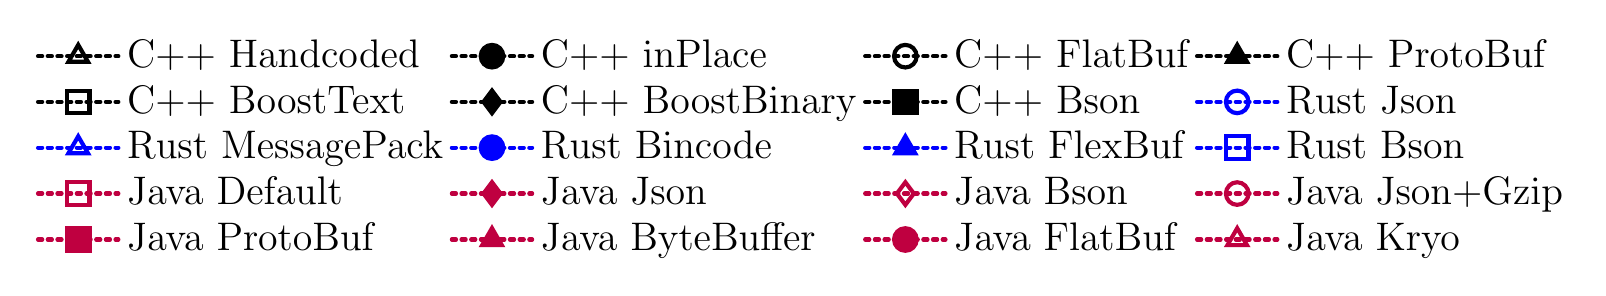
\begin{tikzpicture} 
    \begin{axis}[%
    hide axis,
    xmin=10,
    xmax=50,
    ymin=0,
    ymax=0.4, 
    legend columns=4,
    legend style={draw=white!15!black,legend cell align=left},
    legend style={draw=none, nodes={scale=1.2, transform shape,}, font=\large},    
    legend image post style={line width=1.5pt,scale=1.7},
    legend cell align={left},   
    %/tikz/every even column/.append style={column sep=1.5em},
    ]
    \addlegendimage{black,mark=triangle,dotted, line cap=round,mark options={scale=1.2,solid}}
    \addlegendentry{C++ Handcoded};
    \addlegendimage{black,mark=*,dotted, line cap=round,mark options={scale=1.2,solid}}
    \addlegendentry{C++ inPlace};
    \addlegendimage{black,mark=o,dotted, line cap=round,mark options={scale=1.2,solid}}
    \addlegendentry{C++ FlatBuf};
    \addlegendimage{black,mark=triangle*,dotted, line cap=round,mark options={scale=1.2,solid}}
    \addlegendentry{C++ ProtoBuf};
    \addlegendimage{black,mark=square,dotted, line cap=round,mark options={scale=1.2,solid}}
    \addlegendentry{C++ BoostText};
    \addlegendimage{black,mark=diamond*,dotted, line cap=round,mark options={scale=1.2,solid}}
    \addlegendentry{C++ BoostBinary};
    \addlegendimage{black,mark=square*,dotted, line cap=round,mark options={scale=1.2,solid}}
    \addlegendentry{C++ Bson};

    \addlegendimage{blue,mark=o,dotted, line cap=round,mark options={scale=1.2,solid}}
    \addlegendentry{Rust Json};    
    \addlegendimage{blue,mark=triangle,dotted, line cap=round,mark options={scale=1.2,solid}}
    \addlegendentry{Rust MessagePack};    
    \addlegendimage{blue,mark=*,dotted, line cap=round,mark options={scale=1.2,solid}}
    \addlegendentry{Rust Bincode};    
    \addlegendimage{blue,mark=triangle*,dotted, line cap=round,mark options={scale=1.2,solid}}
    \addlegendentry{Rust FlexBuf};
    \addlegendimage{blue,mark=square,dotted, line cap=round,mark options={scale=1.2,solid}}
    \addlegendentry{Rust Bson};

    \addlegendimage{purple,mark=square,dotted, line cap=round,mark options={scale=1.2,solid}}
    \addlegendentry{Java Default};
    \addlegendimage{purple,mark=diamond*,dotted, line cap=round,mark options={scale=1.2,solid}}
    \addlegendentry{Java Json};
    \addlegendimage{purple,mark=diamond,dotted, line cap=round,mark options={scale=1.2,solid}}
    \addlegendentry{Java Bson};     
    \addlegendimage{purple,mark=o,dotted, line cap=round,mark options={scale=1.2,solid}}
    \addlegendentry{Java Json+Gzip};
    \addlegendimage{purple,mark=square*,dotted, line cap=round,mark options={scale=1.2,solid}}
    \addlegendentry{Java ProtoBuf};
    \addlegendimage{purple,mark=triangle*,dotted, line cap=round,mark options={scale=1.2,solid}}
    \addlegendentry{Java ByteBuffer};
    \addlegendimage{purple,mark=*,dotted, line cap=round,mark options={scale=1.2,solid}}
    \addlegendentry{Java FlatBuf};
    \addlegendimage{purple,mark=triangle,dotted, line cap=round,mark options={scale=1.2,solid}}
    \addlegendentry{Java Kryo};
    
    \end{axis}
\end{tikzpicture}
%         \caption{Experiment2: Parallel (legend)}
% \end{figure*}

% \tikzsetnextfilename{Exp5_network}
%     \begin{figure*}[h]
%         \centering
%         \makeatletter
\newcommand\resetstackedplots{
	\makeatletter
	\pgfplots@stacked@isfirstplottrue
	\makeatother
	\addplot [forget plot,draw=none] coordinates{({HandcodedCPP},0.01) ({inPlaceCPP},0.01) ({FlatBufCPP},0.01) ({ProtoBufCPP},0.01) 
	({BoostCPP},0.01) ({BsonCPP},0.01) ({MessagePackRust},0.01) ({BincodeRust},0.01) ({JsonRust},0.01) ({FlexBufRust},0.01) ({BsonRust},0.01) ({Json+GzipJava},0.01) 
	({JsonJava},0.01) ({BsonJava},0.01) ({DefaultJava},0.01) ({ProtoBufJava},0.01) ({ByteBufferJava},0.01) ({FlatBufJava},0.01) ({KryoJava},0.01)};
}
\makeatother

\begin{tikzpicture}
	\newcommand{\myaddplot}[7]{
	   \addplot[white,xshift=#1,draw=#4,line width=0.15pt, fill=#2, discard if single={#3}{#7}, postaction={pattern=#5,pattern color=#4}] 
	   table[ y=time, col sep=comma, x=baseline] {results/Exp5_network.dat};
	   \label{#3#7}
   };  

   \newcommand{\myaddplotnan}[8]{
	   \addplot[xshift=#1,draw=#8,line width=0.15pt, fill=#2, discard if single={#3}{#7},
	   visualization depends on={value \thisrow{baseline} \as \xbaseline},
	   every node near coord/.append style={		  
		   check for zeronan/.code={
			   \pgfkeys{/pgf/fpu=true}
			   \showvalue{\xbaseline}{inPlaceCPP}{}{}{}{}{}{}{}{}
			   \pgfkeys{/pgf/fpu=false}
		   },
		   check for zeronan,
	   }  
	   ] 
	   table[ y=time, col sep=comma, x=baseline] {results/Exp5_network.dat};	  
	   \label{#3#7}
   };  
   
   \newcommand{\myaddplots}[5]{	   
	\addplot[xshift=#1,draw=#4,line width=0.15pt, fill=#2, discard if single={#3}{#5},
		forget plot,
		nodes near coords custom=1,
		nodes near coords={\pgfmathprintnumber[precision=1]{\pgfplotspointmeta}},
		every node near coord/.append style={
			black,			
			xshift=-5pt,
			anchor=west
		}
	] 
	table[ y=time, col sep=comma, x=baseline] {results/Exp5_network.dat};	
   };   
   
   \newcommand{\addDiagramExpOne}[7]{	
	\nextgroupplot[
		width=#4,				
		ytick=#5,
		yticklabels=#6,
		#7
		]
		\resetstackedplots	
		\myaddplot{0}{#2}{IO}{#2}{none}{I/O Time(taskset True)}{#1};
  		\myaddplotnan{0}{#2!25}{CPU}{#2!25}{north east lines}{CPU Time(taskset True)}{#1}{#2};
		\myaddplots{0}{white}{Total}{none}{#1};
   };     

  \pgfplotsset{
	   discard if single/.style n args={2}{
		   x filter/.code={
		   \edef\tempe{\thisrow{execution}}
		   \edef\tempf{#1}
		   \ifx\tempe\tempf	
			   \edef\tempg{\thisrow{language}}
			   \edef\temph{#2}
			   \ifx\tempg\temph					      
			   \else
			   \def\pgfmathresult{inf}
			   \fi      
		   \else
		   \def\pgfmathresult{inf}
		   \fi      
	   }
	   },
	   nodes near coords custom/.style={
		large value/.style={                    
			rotate=90,
			anchor=east,			
		},
		small value/.style={
			rotate=90,
			anchor=east,
		},
		every node near coord/.style={
		  font=\scriptsize,
		  inner sep=0.5mm,
		  /pgf/number format/1000 sep={},
		  check for zero/.code={%
			\pgfkeys{/pgf/fpu=true}
			\pgfmathparse{\pgfplotspointmeta-0.01}
			\pgfmathfloatifflags{\pgfmathresult}{0}{
				\pgfkeys{/tikz/coordinate}
			}{
				\begingroup                      
					\pgfkeys{/pgf/fpu}%
					\pgfmathparse{\pgfplotspointmeta<#1}%
					\global\let\result=\pgfmathresult
				\endgroup
				\pgfmathfloatcreate{1}{0.01}{0}%
				\let\ONE=\pgfmathresult
				\ifx\result\ONE
					% AH : our condition 'y < #1' is met.
					\pgfkeysalso{/pgfplots/small value}%
				\else
					% ok, proceed as usual.
					\pgfkeysalso{/pgfplots/large value}%
				\fi
			}
			\pgfkeys{/pgf/fpu=false}
		  },
		  check for zero,
		},
	},   
   };
   %%%%%%%%%%%%%%%%%%%%%%%%%%%%%%%%%%%%%%%%%%%%%%%%
   \begin{groupplot}[
		group style={
			group size=3 by 1,
			xlabels at=edge bottom,
			ylabels at=edge left,
			horizontal sep=4pt,
			vertical sep=0pt,
			/pgf/bar width=10pt
		},			
		axis line style={gray},
		ybar stacked,        
		ymode=log,
		ymin=0.1,
		x tick label style={/pgf/number format/1000 sep=},
		ymax=1000,		
		scaled y ticks=false,		  
		enlarge y limits={0.17,upper},		
		ylabel={Execution Time[min]},		   
		ytick align=inside,
		xtick align=outside,			
		xtick pos=left,
		ytick pos=left,
		yticklabel style = {font=\scriptsize},
		ylabel style = {font=\scriptsize, yshift=-12pt},
		xticklabel style = {font=\scriptsize, rotate=50, anchor=east, xshift=1pt, yshift=-1pt},
		x label style={yshift=-20pt},
		xtick=data,
		height=0.55\columnwidth,  
		symbolic x coords={ HandcodedCPP, inPlaceCPP, FlatBufCPP, ProtoBufCPP, BoostCPP, BsonCPP, MessagePackRust, BincodeRust, JsonRust, FlexBufRust, BsonRust, Json+GzipJava, JsonJava, BsonJava, DefaultJava, ProtoBufJava, ByteBufferJava, FlatBufJava, KryoJava},		   
		xticklabels={Handcoded, inPlace, FlatBuf, ProtoBuf, Boost, Bson, MessagePack, Bincode, Json, FlexBuf, Bson, Json+Gzip, Json, Bson, Default, ProtoBuf, ByteBuffer, FlatBuf, Kryo},  		   
		point meta=rawy,            
		nodes near coords={%
    		\pgfmathprintnumberto[fixed,assume math mode=true,precision=1]{\pgfplotspointmeta}{\myval}%
    		\pgfmathparse{\myval<=0.1?:\myval}\pgfmathresult%
		},
		nodes near coords custom={1}, 
		legend image code/.code={\draw [#1] (0cm,-0.1cm) rectangle (0.20cm,0.20cm); },
		xticklabel style={name=T\ticknum}			
]
\addDiagramExpOne{CPP}{black}{white}{0.23\textwidth}{{10,100,1000}}{{10,100,1000}}{{enlarge x limits=0.15,}};	
\node [draw=none,inner sep=3, fill=lightgray!50, text width=0.134\textwidth,align=center,font=\scriptsize, anchor=west](leg1) at (rel axis cs: 0.00,0.955) {C++};

\addDiagramExpOne{Rust}{black}{color7}{0.21\textwidth}{}{}{{enlarge x limits=0.18,}};
\node [draw=none,inner sep=3, fill=lightgray!50, text width=0.134\textwidth,align=center,font=\scriptsize, anchor=west](leg1) at (rel axis cs: 0.00,0.955) {Rust};

\addDiagramExpOne{Java}{black}{color7}{0.29\textwidth}{}{}{{enlarge x limits=0.14,}};
\node [draw=none,inner sep=3, fill=lightgray!50, text width=0.2\textwidth,align=center,font=\scriptsize, anchor=west](leg1) at (rel axis cs: 0.00,0.955) {Java};


\end{groupplot}

\node [draw=none,inner sep=0, font=\scriptsize, anchor=west](leg1) at ($(group c2r1.north west) + (-0.5cm,0.3cm)$) {\shortstack[l]{
		\ref{CPUJava} CPU \ \ \  
		\ref{IOJava} I/O (HDD + Network)
}};


\end{tikzpicture}
%         \caption{Experiment5: (Network)}
% \end{figure*}


% \tikzsetnextfilename{Exp4_externalsort}
%     \begin{figure*}[h]
%         \centering
%         \makeatletter
\newcommand\resetstackedplots{
	\makeatletter
	\pgfplots@stacked@isfirstplottrue
	\makeatother
	\addplot [forget plot,draw=none] coordinates{({HandcodedCPP},0.1) ({inPlaceCPP},0.1) ({FlatBufCPP},0.1) ({ProtoBufCPP},0.1) ({BoostCPP},0.1) ({BsonCPP},0.1) ({MessagePackRust},0.1) ({BincodeRust},0.1) ({JsonRust},0.1) ({FlexBufRust},0.1) ({BsonRust},0.1) ({Json+GzipJava},0.1) ({JsonJava},0.1) ({BsonJava},0.1) ({DefaultJava},0.1) ({ProtoBufJava},0.1) ({ByteBufferJava},0.1) ({FlatBufJava},0.1) ({KryoJava},0.1)};
}
\makeatother


\begin{tikzpicture}
	\newcommand{\myaddplot}[8]{
	   \addplot[white,xshift=#2,draw=#5,line width=0.15pt, fill=#3, discard if single={#1}{#4}{#8}, postaction={pattern=#6,pattern color=#5}] 
	   %\addplot[xshift=#2,draw=#5,line width=0.15pt, discard if single={#1}{#4}{#8}, postaction={pattern=north east lines,pattern color=black}] 
	   table[ y=time, col sep=comma, x=baseline] {results/Exp4_externalsort.dat};
	   \label{#4#1}
   };  

   \newcommand{\myaddplotnan}[9]{
	   \addplot[xshift=#2,draw=#9,line width=0.15pt, fill=#3, discard if single={#1}{#4}{#8}, %postaction={pattern=#6,pattern color=#5},
	   visualization depends on={value \thisrow{baseline} \as \xbaseline},
	   every node near coord/.append style={		  
		   check for zeronan/.code={
			   \pgfkeys{/pgf/fpu=true}
			   \showvalue{\xbaseline}{MessagePackRust}{inPlaceCPP}{JsonRust}{FlatBufJava}{FlexBufRust}{BincodeRust}{}{}{}
			   \pgfkeys{/pgf/fpu=false}
		   },
		   check for zeronan,
	   }  
	   ] 
	   table[ y=time, col sep=comma, x=baseline] {results/Exp4_externalsort.dat};	  
	   \label{#4#1}
   };  
   
   \newcommand{\myaddplots}[6]{	   
	\addplot[xshift=#2,draw=#5,line width=0.15pt, fill=#3, discard if single={#1}{#4}{#6},
		forget plot,
		nodes near coords custom=1,
		nodes near coords={\pgfmathprintnumber[precision=2]{\pgfplotspointmeta}},
		every node near coord/.append style={
			black,			
			xshift=-7pt,
			anchor=west
		}
	] 
	table[ y=time, col sep=comma, x=baseline] {results/Exp4_externalsort.dat};	
   };   
   
   \newcommand{\addDiagramExpOne}[9]{	
	\nextgroupplot[
		width=#4,		
		ytick=#5,
		y axis line style={opacity=#6},
		#7,
		axis y line*=#8,
		%xlabel=#9,				
		]
		\resetstackedplots	
		\myaddplot{True}{-6}{black}{IO}{black}{none}{I/O Time(taskset True)}{#1};
  		\myaddplotnan{True}{-6}{white}{CPU}{black}{north east lines}{CPU Time(taskset True)}{#1}{black};
		\myaddplots{True}{-6}{white}{Total}{none}{#1};
	    \resetstackedplots	 
		\myaddplot{False}{6}{gray!135}{IO}{gray!135}{none}{I/O Time(taskset False)}{#1};  
	    \myaddplotnan{False}{6}{lightgray!85}{CPU}{lightgray!85}{north west lines}{CPU Time(taskset False)}{#1}{black};
		\myaddplots{False}{6}{white}{Total}{none}{#1};    
   };     

  \pgfplotsset{
	   discard if single/.style n args={3}{
		   x filter/.code={
			   \edef\tempa{\thisrow{taskset}}
			   \edef\tempb{#1}
			   \ifx\tempa\tempb
					   \edef\tempe{\thisrow{execution}}
					   \edef\tempf{#2}
					   \ifx\tempe\tempf	
					   	%%%%%%%%%%%%%%%%%%%
						   \edef\tempg{\thisrow{language}}
						   \edef\temph{#3}
						   \ifx\tempg\temph							   		
						   \else
						   \def\pgfmathresult{inf}
						   \fi      
						%%%%%%%%%%%%%%%%%%%	
					   \else
					   \def\pgfmathresult{inf}
					   \fi      
			   \else
			   \def\pgfmathresult{inf}
			   \fi			
		   }
	   },
	   nodes near coords custom/.style={
		large value/.style={                    
			rotate=90,
			anchor=east,			
		},
		small value/.style={
			rotate=90,
			anchor=east,
		},
		every node near coord/.style={
		  font=\scriptsize,
		  inner sep=0.5mm,
		  /pgf/number format/1000 sep={},
		  check for zero/.code={%
			\pgfkeys{/pgf/fpu=true}
			\pgfmathparse{\pgfplotspointmeta-1}
			\pgfmathfloatifflags{\pgfmathresult}{0}{
				\pgfkeys{/tikz/coordinate}
			}{
				\begingroup                      
					\pgfkeys{/pgf/fpu}%
					\pgfmathparse{\pgfplotspointmeta<#1}%
					\global\let\result=\pgfmathresult
				\endgroup
				\pgfmathfloatcreate{1}{1.0}{0}%
				\let\ONE=\pgfmathresult
				\ifx\result\ONE
					% AH : our condition 'y < #1' is met.
					\pgfkeysalso{/pgfplots/small value}%
				\else
					% ok, proceed as usual.
					\pgfkeysalso{/pgfplots/large value}%
				\fi
			}
			\pgfkeys{/pgf/fpu=false}
		  },
		  check for zero,
		},
	},   
   };
   %%%%%%%%%%%%%%%%%%%%%%%%%%%%%%%%%%%%%%%%%%%%%%%%
   \begin{groupplot}[
		group style={
			group size=3 by 1,
			xlabels at=edge bottom,
			ylabels at=edge left,
			horizontal sep=0pt,
			vertical sep=0pt,
			/pgf/bar width=12pt
		},			
		axis line style={gray},
		ybar stacked,        
		ymode=log,
		ymin=0.55,
		ymax=270,
		scaled y ticks=false,		  
		enlarge y limits={0.5,upper},		
		ylabel={Execution Time[min.]},		   
		ytick align=inside,
		xtick align=outside,			
		xtick pos=left,
		ytick pos=left,
		yticklabel style = {font=\scriptsize},
		ylabel style = {font=\scriptsize, yshift=-12pt},
		xticklabel style = {font=\scriptsize},
		x label style={yshift=-20pt},
		xtick=data,
		height=0.6\columnwidth,  
		symbolic x coords={ HandcodedCPP, inPlaceCPP, FlatBufCPP, ProtoBufCPP, BoostCPP, BsonCPP, MessagePackRust, BincodeRust, JsonRust, FlexBufRust, BsonRust, Json+GzipJava, JsonJava, BsonJava, DefaultJava, ProtoBufJava, ByteBufferJava, FlatBufJava, KryoJava},		   
		xticklabels={ HandCoded,, FlatBuf,, Boost,, MessagePack,, Json,, Bson,, Json,, Default,, Byte Buffer,, Kryo},  
		extra x ticks={inPlaceCPP,ProtoBufCPP,BsonCPP,BincodeRust,FlexBufRust,Json+GzipJava,BsonJava, ProtoBufJava,FlatBufJava},
		extra x tick labels={inPlace,ProtoBuf,Bson,Bincode,FlexBuf,Json+Gzip,Bson,ProtoBuf,FlatBuf},
		every extra x tick/.style={major tick length=15pt, xtick align=outside},
		point meta=rawy,            
		nodes near coords={\pgfmathprintnumber[precision=1]{\pgfplotspointmeta}},
		nodes near coords custom={1}, 
		legend image code/.code={\draw [#1] (0cm,-0.1cm) rectangle (0.20cm,0.20cm); },
		xticklabel style={name=T\ticknum}			
]
\addDiagramExpOne{CPP}{tugb}{color7}{0.42\textwidth}{{0,10,100,1000}}{1}{{enlarge x limits=0.12,}}{left}{C++};		

\node [draw=none,inner sep=0, font=\scriptsize, anchor=west](leg1) at (rel axis cs: 0.04,0.85) {\shortstack[l]{
		\ref{CPUTrue} CPU Time(taskset True) \\ \\
		\ref{IOTrue} I/O Time(taskset True) 			
}};
\addDiagramExpOne{Rust}{tugb}{color7}{0.40\textwidth}{\empty}{0}{{enlarge x limits=0.24,}}{left}{Rust};
\node [draw=none,inner sep=0, font=\scriptsize, anchor=west](leg1) at (rel axis cs: 0.04,0.85) {\shortstack[l]{
		\ref{CPUFalse} CPU Time(taskset False) \\ \\
		\ref{IOFalse} I/O Time(taskset False) 			
}};
\addDiagramExpOne{Java}{tugb}{color7}{0.53\textwidth}{\empty}{1}{{enlarge x limits=0.12,}}{right}{Java};
		
\end{groupplot}

\begin{scope}[decoration=brace]
	\pgfdecorationsegmentamplitude=5pt
	\draw[decorate] ($(T2.south east)+(-5pt,0)$) -- ($(T0.south west)+(-20pt,0)$) node[midway,below=\pgfdecorationsegmentamplitude] {\footnotesize{C++}};
	\draw[decorate] ($(T4.south east)+(20pt,0)$) -- ($(T3.south west)+(-25pt,0)$) node[midway,below=\pgfdecorationsegmentamplitude] {\footnotesize{Rust}};
	\draw[decorate] ($(T8.south east)+(20pt,0)$) -- ($(T5.south west)+(-0pt,0)$) node[midway,below=\pgfdecorationsegmentamplitude] {\footnotesize{Java}};	
  \end{scope}
\end{tikzpicture}
%         \caption{Experiment4: (Externalsort)}
% \end{figure*}


\maketitle
\IEEEdisplaynontitleabstractindextext
\IEEEpeerreviewmaketitle
\bibliographystyle{IEEEtran}
\bibliography{References}

\end{document}